\documentclass[twoside]{book}

% Packages required by doxygen
\usepackage{fixltx2e}
\usepackage{calc}
\usepackage{doxygen}
\usepackage[export]{adjustbox} % also loads graphicx
\usepackage{graphicx}
\usepackage[utf8]{inputenc}
\usepackage{makeidx}
\usepackage{multicol}
\usepackage{multirow}
\PassOptionsToPackage{warn}{textcomp}
\usepackage{textcomp}
\usepackage[nointegrals]{wasysym}
\usepackage[table]{xcolor}

% NLS support packages
\usepackage[french]{babel}

% Font selection
\usepackage[T1]{fontenc}
\usepackage[scaled=.90]{helvet}
\usepackage{courier}
\usepackage{amssymb}
\usepackage{sectsty}
\renewcommand{\familydefault}{\sfdefault}
\allsectionsfont{%
  \fontseries{bc}\selectfont%
  \color{darkgray}%
}
\renewcommand{\DoxyLabelFont}{%
  \fontseries{bc}\selectfont%
  \color{darkgray}%
}
\newcommand{\+}{\discretionary{\mbox{\scriptsize$\hookleftarrow$}}{}{}}

% Page & text layout
\usepackage{geometry}
\geometry{%
  a4paper,%
  top=2.5cm,%
  bottom=2.5cm,%
  left=2.5cm,%
  right=2.5cm%
}
\tolerance=750
\hfuzz=15pt
\hbadness=750
\setlength{\emergencystretch}{15pt}
\setlength{\parindent}{0cm}
\setlength{\parskip}{3ex plus 2ex minus 2ex}
\makeatletter
\renewcommand{\paragraph}{%
  \@startsection{paragraph}{4}{0ex}{-1.0ex}{1.0ex}{%
    \normalfont\normalsize\bfseries\SS@parafont%
  }%
}
\renewcommand{\subparagraph}{%
  \@startsection{subparagraph}{5}{0ex}{-1.0ex}{1.0ex}{%
    \normalfont\normalsize\bfseries\SS@subparafont%
  }%
}
\makeatother

% Headers & footers
\usepackage{fancyhdr}
\pagestyle{fancyplain}
\fancyhead[LE]{\fancyplain{}{\bfseries\thepage}}
\fancyhead[CE]{\fancyplain{}{}}
\fancyhead[RE]{\fancyplain{}{\bfseries\leftmark}}
\fancyhead[LO]{\fancyplain{}{\bfseries\rightmark}}
\fancyhead[CO]{\fancyplain{}{}}
\fancyhead[RO]{\fancyplain{}{\bfseries\thepage}}
\fancyfoot[LE]{\fancyplain{}{}}
\fancyfoot[CE]{\fancyplain{}{}}
\fancyfoot[RE]{\fancyplain{}{\bfseries\scriptsize Généré par Doxygen }}
\fancyfoot[LO]{\fancyplain{}{\bfseries\scriptsize Généré par Doxygen }}
\fancyfoot[CO]{\fancyplain{}{}}
\fancyfoot[RO]{\fancyplain{}{}}
\renewcommand{\footrulewidth}{0.4pt}
\renewcommand{\chaptermark}[1]{%
  \markboth{#1}{}%
}
\renewcommand{\sectionmark}[1]{%
  \markright{\thesection\ #1}%
}

% Indices & bibliography
\usepackage{natbib}
\usepackage[titles]{tocloft}
\setcounter{tocdepth}{3}
\setcounter{secnumdepth}{5}
\makeindex

% Hyperlinks (required, but should be loaded last)
\usepackage{ifpdf}
\ifpdf
  \usepackage[pdftex,pagebackref=true]{hyperref}
\else
  \usepackage[ps2pdf,pagebackref=true]{hyperref}
\fi
\hypersetup{%
  colorlinks=true,%
  linkcolor=blue,%
  citecolor=blue,%
  unicode%
}

% Custom commands
\newcommand{\clearemptydoublepage}{%
  \newpage{\pagestyle{empty}\cleardoublepage}%
}

\usepackage{caption}
\captionsetup{labelsep=space,justification=centering,font={bf},singlelinecheck=off,skip=4pt,position=top}

%===== C O N T E N T S =====

\begin{document}

% Titlepage & ToC
\hypersetup{pageanchor=false,
             bookmarksnumbered=true,
             pdfencoding=unicode
            }
\pagenumbering{roman}
\begin{titlepage}
\vspace*{7cm}
\begin{center}%
{\Large Gestion\+Serre \\[1ex]\large 1.\+1 }\\
\vspace*{1cm}
{\large Généré par Doxygen 1.8.11}\\
\end{center}
\end{titlepage}
\clearemptydoublepage
\tableofcontents
\clearemptydoublepage
\pagenumbering{arabic}
\hypersetup{pageanchor=true}

%--- Begin generated contents ---
\chapter{Index des classes}
\section{Liste des classes}
Liste des classes, structures, unions et interfaces avec une brève description \+:\begin{DoxyCompactList}
\item\contentsline{section}{\hyperlink{class_controleur_de_serre}{Controleur\+De\+Serre} }{\pageref{class_controleur_de_serre}}{}
\item\contentsline{section}{\hyperlink{class_humidite}{Humidite} }{\pageref{class_humidite}}{}
\item\contentsline{section}{\hyperlink{class_timer}{Timer} }{\pageref{class_timer}}{}
\item\contentsline{section}{\hyperlink{class_vanne}{Vanne} }{\pageref{class_vanne}}{}
\item\contentsline{section}{\hyperlink{class_zone}{Zone} }{\pageref{class_zone}}{}
\end{DoxyCompactList}

\chapter{Index des fichiers}
\section{Liste des fichiers}
Liste de tous les fichiers avec une brève description \+:\begin{DoxyCompactList}
\item\contentsline{section}{\hyperlink{controleur_de_serre_8cpp}{controleur\+De\+Serre.\+cpp} }{\pageref{controleur_de_serre_8cpp}}{}
\item\contentsline{section}{\hyperlink{controleur_de_serre_8h}{controleur\+De\+Serre.\+h} }{\pageref{controleur_de_serre_8h}}{}
\item\contentsline{section}{\hyperlink{humidite_8cpp}{humidite.\+cpp} }{\pageref{humidite_8cpp}}{}
\item\contentsline{section}{\hyperlink{humidite_8h}{humidite.\+h} }{\pageref{humidite_8h}}{}
\item\contentsline{section}{\hyperlink{timer_8cpp}{timer.\+cpp} }{\pageref{timer_8cpp}}{}
\item\contentsline{section}{\hyperlink{timer_8h}{timer.\+h} }{\pageref{timer_8h}}{}
\item\contentsline{section}{\hyperlink{vanne_8cpp}{vanne.\+cpp} }{\pageref{vanne_8cpp}}{}
\item\contentsline{section}{\hyperlink{vanne_8h}{vanne.\+h} }{\pageref{vanne_8h}}{}
\item\contentsline{section}{\hyperlink{zone_8cpp}{zone.\+cpp} }{\pageref{zone_8cpp}}{}
\item\contentsline{section}{\hyperlink{zone_8h}{zone.\+h} }{\pageref{zone_8h}}{}
\end{DoxyCompactList}

\chapter{Documentation des classes}
\hypertarget{class_controleur_de_serre}{}\section{Référence de la classe Controleur\+De\+Serre}
\label{class_controleur_de_serre}\index{Controleur\+De\+Serre@{Controleur\+De\+Serre}}


{\ttfamily \#include $<$controleur\+De\+Serre.\+h$>$}



Graphe de collaboration de Controleur\+De\+Serre\+:\nopagebreak
\begin{figure}[H]
\begin{center}
\leavevmode
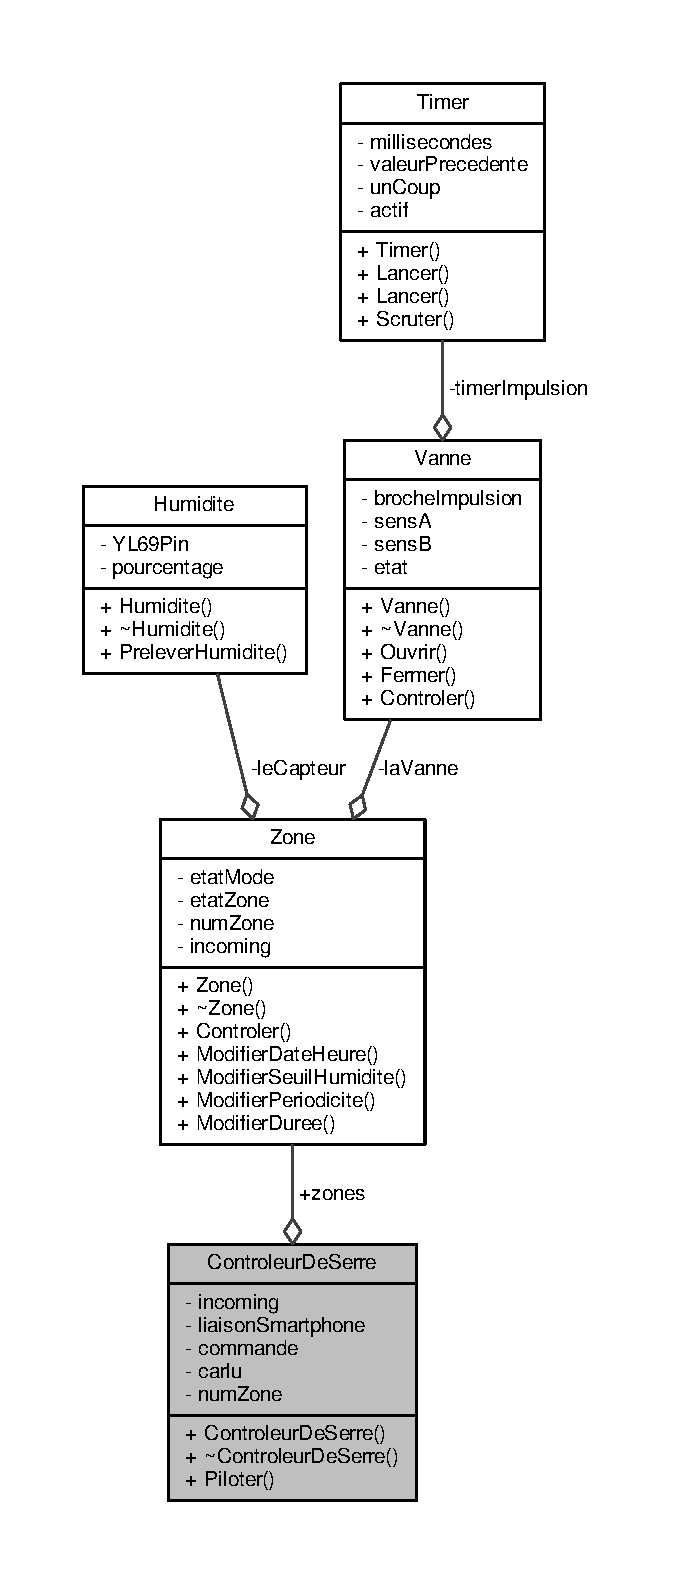
\includegraphics[height=550pt]{class_controleur_de_serre__coll__graph}
\end{center}
\end{figure}
\subsection*{Fonctions membres publiques}
\begin{DoxyCompactItemize}
\item 
\hyperlink{class_controleur_de_serre_afe055fb82c48b1c58575bba396d8d09f}{Controleur\+De\+Serre} ()
\item 
\hyperlink{class_controleur_de_serre_a657ac6eb145dacc226d9de1adaa9b2ab}{$\sim$\+Controleur\+De\+Serre} ()
\item 
void \hyperlink{class_controleur_de_serre_ab2b0f97cc39a24b330e214901f1c1323}{Piloter} ()
\end{DoxyCompactItemize}
\subsection*{Attributs publics}
\begin{DoxyCompactItemize}
\item 
\hyperlink{class_zone}{Zone} $\ast$ \hyperlink{class_controleur_de_serre_ad0cfc26f13ccea8cc304763caa32d3a5}{zones} \mbox{[}4\mbox{]}
\end{DoxyCompactItemize}
\subsection*{Attributs privés}
\begin{DoxyCompactItemize}
\item 
String \hyperlink{class_controleur_de_serre_aff14cbd8c5c61d76d592922ad81264d8}{incoming}
\item 
Bluetooth\+Serial \hyperlink{class_controleur_de_serre_a256aa95390c10b20876951613411372d}{liaison\+Smartphone}
\item 
char \hyperlink{class_controleur_de_serre_adfb41079ae94c40c8eaeb784b485c018}{commande}
\item 
char \hyperlink{class_controleur_de_serre_a193c19856f0c0b34cd405eabce6ddfab}{carlu}
\item 
char \hyperlink{class_controleur_de_serre_a743d1b27b4f77a807a199ef418a236d4}{num\+Zone}
\end{DoxyCompactItemize}


\subsection{Documentation des constructeurs et destructeur}
\index{Controleur\+De\+Serre@{Controleur\+De\+Serre}!Controleur\+De\+Serre@{Controleur\+De\+Serre}}
\index{Controleur\+De\+Serre@{Controleur\+De\+Serre}!Controleur\+De\+Serre@{Controleur\+De\+Serre}}
\subsubsection[{\texorpdfstring{Controleur\+De\+Serre()}{ControleurDeSerre()}}]{\setlength{\rightskip}{0pt plus 5cm}Controleur\+De\+Serre\+::\+Controleur\+De\+Serre (
\begin{DoxyParamCaption}
{}
\end{DoxyParamCaption}
)}\hypertarget{class_controleur_de_serre_afe055fb82c48b1c58575bba396d8d09f}{}\label{class_controleur_de_serre_afe055fb82c48b1c58575bba396d8d09f}
\hyperlink{class_controleur_de_serre}{Controleur\+De\+Serre}

Constructeur de la classe, on va initialiser dans un tableau nos différentes zones ici 4 et on va démarrer la liaison bluetooth. \index{Controleur\+De\+Serre@{Controleur\+De\+Serre}!````~Controleur\+De\+Serre@{$\sim$\+Controleur\+De\+Serre}}
\index{````~Controleur\+De\+Serre@{$\sim$\+Controleur\+De\+Serre}!Controleur\+De\+Serre@{Controleur\+De\+Serre}}
\subsubsection[{\texorpdfstring{$\sim$\+Controleur\+De\+Serre()}{~ControleurDeSerre()}}]{\setlength{\rightskip}{0pt plus 5cm}Controleur\+De\+Serre\+::$\sim$\+Controleur\+De\+Serre (
\begin{DoxyParamCaption}
{}
\end{DoxyParamCaption}
)}\hypertarget{class_controleur_de_serre_a657ac6eb145dacc226d9de1adaa9b2ab}{}\label{class_controleur_de_serre_a657ac6eb145dacc226d9de1adaa9b2ab}
\+::$\sim$\+Controleur\+De\+Serre

Déstructeur de la classe, on va venir supprimer, effacer les zones crées dans le constructeur. 

\subsection{Documentation des fonctions membres}
\index{Controleur\+De\+Serre@{Controleur\+De\+Serre}!Piloter@{Piloter}}
\index{Piloter@{Piloter}!Controleur\+De\+Serre@{Controleur\+De\+Serre}}
\subsubsection[{\texorpdfstring{Piloter()}{Piloter()}}]{\setlength{\rightskip}{0pt plus 5cm}void Controleur\+De\+Serre\+::\+Piloter (
\begin{DoxyParamCaption}
{}
\end{DoxyParamCaption}
)}\hypertarget{class_controleur_de_serre_ab2b0f97cc39a24b330e214901f1c1323}{}\label{class_controleur_de_serre_ab2b0f97cc39a24b330e214901f1c1323}
\hyperlink{class_controleur_de_serre}{Controleur\+De\+Serre}

Première Partie \+: Tant que la liaison bluetooth fonctionne on récupére la chaine de caractère envoyée

Deuxième Partie \+: On compare la chaine de caractère, si le premier caractère est un z on regarde le deuxième pour obtenir le numéro de la zone. puis on appelle la méthode Controler (). 

\subsection{Documentation des données membres}
\index{Controleur\+De\+Serre@{Controleur\+De\+Serre}!carlu@{carlu}}
\index{carlu@{carlu}!Controleur\+De\+Serre@{Controleur\+De\+Serre}}
\subsubsection[{\texorpdfstring{carlu}{carlu}}]{\setlength{\rightskip}{0pt plus 5cm}char Controleur\+De\+Serre\+::carlu\hspace{0.3cm}{\ttfamily [private]}}\hypertarget{class_controleur_de_serre_a193c19856f0c0b34cd405eabce6ddfab}{}\label{class_controleur_de_serre_a193c19856f0c0b34cd405eabce6ddfab}
\index{Controleur\+De\+Serre@{Controleur\+De\+Serre}!commande@{commande}}
\index{commande@{commande}!Controleur\+De\+Serre@{Controleur\+De\+Serre}}
\subsubsection[{\texorpdfstring{commande}{commande}}]{\setlength{\rightskip}{0pt plus 5cm}char Controleur\+De\+Serre\+::commande\hspace{0.3cm}{\ttfamily [private]}}\hypertarget{class_controleur_de_serre_adfb41079ae94c40c8eaeb784b485c018}{}\label{class_controleur_de_serre_adfb41079ae94c40c8eaeb784b485c018}
\index{Controleur\+De\+Serre@{Controleur\+De\+Serre}!incoming@{incoming}}
\index{incoming@{incoming}!Controleur\+De\+Serre@{Controleur\+De\+Serre}}
\subsubsection[{\texorpdfstring{incoming}{incoming}}]{\setlength{\rightskip}{0pt plus 5cm}String Controleur\+De\+Serre\+::incoming\hspace{0.3cm}{\ttfamily [private]}}\hypertarget{class_controleur_de_serre_aff14cbd8c5c61d76d592922ad81264d8}{}\label{class_controleur_de_serre_aff14cbd8c5c61d76d592922ad81264d8}
\index{Controleur\+De\+Serre@{Controleur\+De\+Serre}!liaison\+Smartphone@{liaison\+Smartphone}}
\index{liaison\+Smartphone@{liaison\+Smartphone}!Controleur\+De\+Serre@{Controleur\+De\+Serre}}
\subsubsection[{\texorpdfstring{liaison\+Smartphone}{liaisonSmartphone}}]{\setlength{\rightskip}{0pt plus 5cm}Bluetooth\+Serial Controleur\+De\+Serre\+::liaison\+Smartphone\hspace{0.3cm}{\ttfamily [private]}}\hypertarget{class_controleur_de_serre_a256aa95390c10b20876951613411372d}{}\label{class_controleur_de_serre_a256aa95390c10b20876951613411372d}
\index{Controleur\+De\+Serre@{Controleur\+De\+Serre}!num\+Zone@{num\+Zone}}
\index{num\+Zone@{num\+Zone}!Controleur\+De\+Serre@{Controleur\+De\+Serre}}
\subsubsection[{\texorpdfstring{num\+Zone}{numZone}}]{\setlength{\rightskip}{0pt plus 5cm}char Controleur\+De\+Serre\+::num\+Zone\hspace{0.3cm}{\ttfamily [private]}}\hypertarget{class_controleur_de_serre_a743d1b27b4f77a807a199ef418a236d4}{}\label{class_controleur_de_serre_a743d1b27b4f77a807a199ef418a236d4}
\index{Controleur\+De\+Serre@{Controleur\+De\+Serre}!zones@{zones}}
\index{zones@{zones}!Controleur\+De\+Serre@{Controleur\+De\+Serre}}
\subsubsection[{\texorpdfstring{zones}{zones}}]{\setlength{\rightskip}{0pt plus 5cm}{\bf Zone}$\ast$ Controleur\+De\+Serre\+::zones\mbox{[}4\mbox{]}}\hypertarget{class_controleur_de_serre_ad0cfc26f13ccea8cc304763caa32d3a5}{}\label{class_controleur_de_serre_ad0cfc26f13ccea8cc304763caa32d3a5}


La documentation de cette classe a été générée à partir des fichiers suivants \+:\begin{DoxyCompactItemize}
\item 
\hyperlink{controleur_de_serre_8h}{controleur\+De\+Serre.\+h}\item 
\hyperlink{controleur_de_serre_8cpp}{controleur\+De\+Serre.\+cpp}\end{DoxyCompactItemize}

\hypertarget{class_humidite}{}\section{Référence de la classe Humidite}
\label{class_humidite}\index{Humidite@{Humidite}}


{\ttfamily \#include $<$humidite.\+h$>$}



Graphe de collaboration de Humidite\+:\nopagebreak
\begin{figure}[H]
\begin{center}
\leavevmode
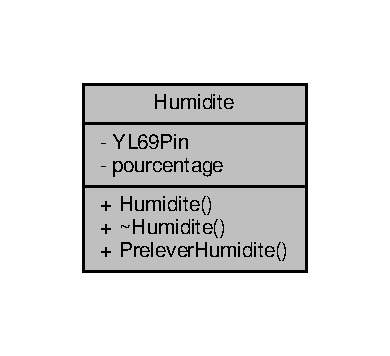
\includegraphics[width=187pt]{class_humidite__coll__graph}
\end{center}
\end{figure}
\subsection*{Fonctions membres publiques}
\begin{DoxyCompactItemize}
\item 
\hyperlink{class_humidite_aca27c2f9386a6c48fae1ac47146282dc}{Humidite} (gpio\+\_\+num\+\_\+t \+\_\+broche\+Mesure)
\begin{DoxyCompactList}\small\item\em \hyperlink{class_humidite_aca27c2f9386a6c48fae1ac47146282dc}{Humidite\+::\+Humidite}. \end{DoxyCompactList}\item 
\hyperlink{class_humidite_ac03560148d13e0d08b7c70fc5878b0a0}{$\sim$\+Humidite} ()
\begin{DoxyCompactList}\small\item\em \hyperlink{class_humidite_ac03560148d13e0d08b7c70fc5878b0a0}{Humidite\+::$\sim$\+Humidite}. \end{DoxyCompactList}\item 
int \hyperlink{class_humidite_abc7c4e7f47a37409ab3ac45402fca85a}{Prelever\+Humidite} ()
\begin{DoxyCompactList}\small\item\em \hyperlink{class_humidite_abc7c4e7f47a37409ab3ac45402fca85a}{Humidite\+::\+Prelever\+Humidite}. \end{DoxyCompactList}\end{DoxyCompactItemize}
\subsection*{Attributs privés}
\begin{DoxyCompactItemize}
\item 
const int \hyperlink{class_humidite_aec11fda83eec67083d5859c314167c08}{Y\+L69\+Pin}
\item 
int \hyperlink{class_humidite_a9811e1cf3bfa87a05312f4d22d2093c8}{pourcentage} = 0
\end{DoxyCompactItemize}


\subsection{Documentation des constructeurs et destructeur}
\index{Humidite@{Humidite}!Humidite@{Humidite}}
\index{Humidite@{Humidite}!Humidite@{Humidite}}
\subsubsection[{\texorpdfstring{Humidite(gpio\+\_\+num\+\_\+t \+\_\+broche\+Mesure)}{Humidite(gpio_num_t _brocheMesure)}}]{\setlength{\rightskip}{0pt plus 5cm}Humidite\+::\+Humidite (
\begin{DoxyParamCaption}
\item[{gpio\+\_\+num\+\_\+t}]{\+\_\+broche\+Mesure}
\end{DoxyParamCaption}
)}\hypertarget{class_humidite_aca27c2f9386a6c48fae1ac47146282dc}{}\label{class_humidite_aca27c2f9386a6c48fae1ac47146282dc}


\hyperlink{class_humidite_aca27c2f9386a6c48fae1ac47146282dc}{Humidite\+::\+Humidite}. 


\begin{DoxyParams}{Paramètres}
{\em gpio\+\_\+num\+\_\+t} & \+\_\+broche\+Mesure c\textquotesingle{}est le numéro de la broche du capteur d\textquotesingle{}humidité\\
\hline
\end{DoxyParams}
Constructeur de la classe \index{Humidite@{Humidite}!````~Humidite@{$\sim$\+Humidite}}
\index{````~Humidite@{$\sim$\+Humidite}!Humidite@{Humidite}}
\subsubsection[{\texorpdfstring{$\sim$\+Humidite()}{~Humidite()}}]{\setlength{\rightskip}{0pt plus 5cm}Humidite\+::$\sim$\+Humidite (
\begin{DoxyParamCaption}
{}
\end{DoxyParamCaption}
)}\hypertarget{class_humidite_ac03560148d13e0d08b7c70fc5878b0a0}{}\label{class_humidite_ac03560148d13e0d08b7c70fc5878b0a0}


\hyperlink{class_humidite_ac03560148d13e0d08b7c70fc5878b0a0}{Humidite\+::$\sim$\+Humidite}. 


\begin{DoxyParams}{Paramètres}
{\em gpio\+\_\+num\+\_\+t} & \+\_\+broche\+Mesure c\textquotesingle{}est le numéro de la broche du capteur d\textquotesingle{}humidité\\
\hline
\end{DoxyParams}
Déstructeur de la classe 

\subsection{Documentation des fonctions membres}
\index{Humidite@{Humidite}!Prelever\+Humidite@{Prelever\+Humidite}}
\index{Prelever\+Humidite@{Prelever\+Humidite}!Humidite@{Humidite}}
\subsubsection[{\texorpdfstring{Prelever\+Humidite()}{PreleverHumidite()}}]{\setlength{\rightskip}{0pt plus 5cm}int Humidite\+::\+Prelever\+Humidite (
\begin{DoxyParamCaption}
{}
\end{DoxyParamCaption}
)}\hypertarget{class_humidite_abc7c4e7f47a37409ab3ac45402fca85a}{}\label{class_humidite_abc7c4e7f47a37409ab3ac45402fca85a}


\hyperlink{class_humidite_abc7c4e7f47a37409ab3ac45402fca85a}{Humidite\+::\+Prelever\+Humidite}. 

On va venir lire le capteur et récuperer le taux d\textquotesingle{}humidité que l\textquotesingle{}on va convertir en pourcentage 

\subsection{Documentation des données membres}
\index{Humidite@{Humidite}!pourcentage@{pourcentage}}
\index{pourcentage@{pourcentage}!Humidite@{Humidite}}
\subsubsection[{\texorpdfstring{pourcentage}{pourcentage}}]{\setlength{\rightskip}{0pt plus 5cm}int Humidite\+::pourcentage = 0\hspace{0.3cm}{\ttfamily [private]}}\hypertarget{class_humidite_a9811e1cf3bfa87a05312f4d22d2093c8}{}\label{class_humidite_a9811e1cf3bfa87a05312f4d22d2093c8}
\index{Humidite@{Humidite}!Y\+L69\+Pin@{Y\+L69\+Pin}}
\index{Y\+L69\+Pin@{Y\+L69\+Pin}!Humidite@{Humidite}}
\subsubsection[{\texorpdfstring{Y\+L69\+Pin}{YL69Pin}}]{\setlength{\rightskip}{0pt plus 5cm}const int Humidite\+::\+Y\+L69\+Pin\hspace{0.3cm}{\ttfamily [private]}}\hypertarget{class_humidite_aec11fda83eec67083d5859c314167c08}{}\label{class_humidite_aec11fda83eec67083d5859c314167c08}


La documentation de cette classe a été générée à partir des fichiers suivants \+:\begin{DoxyCompactItemize}
\item 
\hyperlink{humidite_8h}{humidite.\+h}\item 
\hyperlink{humidite_8cpp}{humidite.\+cpp}\end{DoxyCompactItemize}

\hypertarget{class_timer}{}\section{Référence de la classe Timer}
\label{class_timer}\index{Timer@{Timer}}


{\ttfamily \#include $<$timer.\+h$>$}



Graphe de collaboration de Timer\+:\nopagebreak
\begin{figure}[H]
\begin{center}
\leavevmode
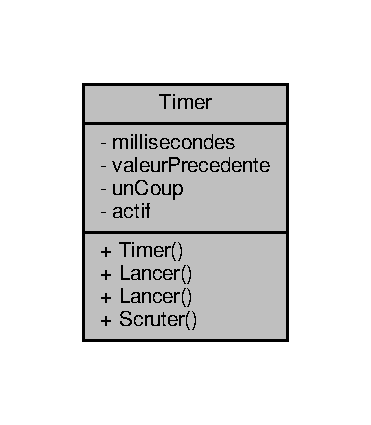
\includegraphics[width=178pt]{class_timer__coll__graph}
\end{center}
\end{figure}
\subsection*{Fonctions membres publiques}
\begin{DoxyCompactItemize}
\item 
\hyperlink{class_timer_a7bbdf7d44a20493674484af45b8f8a98}{Timer} (bool \+\_\+un\+Coup=false)
\begin{DoxyCompactList}\small\item\em \hyperlink{class_timer_a7bbdf7d44a20493674484af45b8f8a98}{Timer\+::\+Timer}. \end{DoxyCompactList}\item 
void \hyperlink{class_timer_a9a30698d13e0369d35307de5d156330f}{Lancer} (unsigned long \+\_\+milli\+Secondes)
\begin{DoxyCompactList}\small\item\em \hyperlink{class_timer_a9a30698d13e0369d35307de5d156330f}{Timer\+::\+Lancer}. \end{DoxyCompactList}\item 
void \hyperlink{class_timer_a17e620ab8d93dd449191b3ced782b153}{Lancer} (int \+\_\+heures, int \+\_\+minutes, int \+\_\+secondes)
\begin{DoxyCompactList}\small\item\em \hyperlink{class_timer_a9a30698d13e0369d35307de5d156330f}{Timer\+::\+Lancer}. \end{DoxyCompactList}\item 
bool \hyperlink{class_timer_aa26129870e5b0a3b2623b70b1412ad7e}{Scruter} ()
\begin{DoxyCompactList}\small\item\em \hyperlink{class_timer_aa26129870e5b0a3b2623b70b1412ad7e}{Timer\+::\+Scruter}. \end{DoxyCompactList}\end{DoxyCompactItemize}
\subsection*{Attributs privés}
\begin{DoxyCompactItemize}
\item 
unsigned long \hyperlink{class_timer_a1423b1f13ea00903f9581020e5d40198}{millisecondes}
\item 
unsigned long \hyperlink{class_timer_aefa4811f3619dc170520bc43c86c36f6}{valeur\+Precedente}
\begin{DoxyCompactList}\small\item\em Durée de l\textquotesingle{}attente. \end{DoxyCompactList}\item 
bool \hyperlink{class_timer_a992bb5566966aba6e82a7f4ebfa90c4f}{un\+Coup}
\begin{DoxyCompactList}\small\item\em valeur du temps précédent \end{DoxyCompactList}\item 
bool \hyperlink{class_timer_aaf1ab0317d3937d55a19cf7fac56818b}{actif}
\begin{DoxyCompactList}\small\item\em Mode du timer vrai une seule fois, faux mode infini. \end{DoxyCompactList}\end{DoxyCompactItemize}


\subsection{Documentation des constructeurs et destructeur}
\index{Timer@{Timer}!Timer@{Timer}}
\index{Timer@{Timer}!Timer@{Timer}}
\subsubsection[{\texorpdfstring{Timer(bool \+\_\+un\+Coup=false)}{Timer(bool _unCoup=false)}}]{\setlength{\rightskip}{0pt plus 5cm}Timer\+::\+Timer (
\begin{DoxyParamCaption}
\item[{bool}]{\+\_\+un\+Coup = {\ttfamily false}}
\end{DoxyParamCaption}
)}\hypertarget{class_timer_a7bbdf7d44a20493674484af45b8f8a98}{}\label{class_timer_a7bbdf7d44a20493674484af45b8f8a98}


\hyperlink{class_timer_a7bbdf7d44a20493674484af45b8f8a98}{Timer\+::\+Timer}. 


\begin{DoxyParams}{Paramètres}
{\em \+\_\+un\+Coup} & permet de définir le mode du timer par défaut mode infini, si true alors une seule fois\\
\hline
\end{DoxyParams}
Constructeur de la classe. Le timer est inactif, il faut appelé Lancer ensuite. 

\subsection{Documentation des fonctions membres}
\index{Timer@{Timer}!Lancer@{Lancer}}
\index{Lancer@{Lancer}!Timer@{Timer}}
\subsubsection[{\texorpdfstring{Lancer(unsigned long \+\_\+milli\+Secondes)}{Lancer(unsigned long _milliSecondes)}}]{\setlength{\rightskip}{0pt plus 5cm}void Timer\+::\+Lancer (
\begin{DoxyParamCaption}
\item[{unsigned long}]{\+\_\+milli\+Secondes}
\end{DoxyParamCaption}
)}\hypertarget{class_timer_a9a30698d13e0369d35307de5d156330f}{}\label{class_timer_a9a30698d13e0369d35307de5d156330f}


\hyperlink{class_timer_a9a30698d13e0369d35307de5d156330f}{Timer\+::\+Lancer}. 


\begin{DoxyParams}{Paramètres}
{\em \+\_\+milli\+Secondes} & Durée de la tempo\\
\hline
\end{DoxyParams}
Lance le timer avec le temps en millisecondes \index{Timer@{Timer}!Lancer@{Lancer}}
\index{Lancer@{Lancer}!Timer@{Timer}}
\subsubsection[{\texorpdfstring{Lancer(int \+\_\+heures, int \+\_\+minutes, int \+\_\+secondes)}{Lancer(int _heures, int _minutes, int _secondes)}}]{\setlength{\rightskip}{0pt plus 5cm}void Timer\+::\+Lancer (
\begin{DoxyParamCaption}
\item[{int}]{\+\_\+heures, }
\item[{int}]{\+\_\+minutes, }
\item[{int}]{\+\_\+secondes}
\end{DoxyParamCaption}
)}\hypertarget{class_timer_a17e620ab8d93dd449191b3ced782b153}{}\label{class_timer_a17e620ab8d93dd449191b3ced782b153}


\hyperlink{class_timer_a9a30698d13e0369d35307de5d156330f}{Timer\+::\+Lancer}. 


\begin{DoxyParams}{Paramètres}
{\em \+\_\+heures} & \\
\hline
{\em \+\_\+minutes} & \\
\hline
{\em \+\_\+secondes} & \\
\hline
\end{DoxyParams}
Lance le timer avec le temps exprimé en heures, minutes, secondes \index{Timer@{Timer}!Scruter@{Scruter}}
\index{Scruter@{Scruter}!Timer@{Timer}}
\subsubsection[{\texorpdfstring{Scruter()}{Scruter()}}]{\setlength{\rightskip}{0pt plus 5cm}bool Timer\+::\+Scruter (
\begin{DoxyParamCaption}
{}
\end{DoxyParamCaption}
)}\hypertarget{class_timer_aa26129870e5b0a3b2623b70b1412ad7e}{}\label{class_timer_aa26129870e5b0a3b2623b70b1412ad7e}


\hyperlink{class_timer_aa26129870e5b0a3b2623b70b1412ad7e}{Timer\+::\+Scruter}. 

\begin{DoxyReturn}{Renvoie}
vrai si le temps est écoulé, faux sinon
\end{DoxyReturn}
Si le timer est configuré pour une seule fois, l\textquotesingle{}attribut actif repasse à faux 

\subsection{Documentation des données membres}
\index{Timer@{Timer}!actif@{actif}}
\index{actif@{actif}!Timer@{Timer}}
\subsubsection[{\texorpdfstring{actif}{actif}}]{\setlength{\rightskip}{0pt plus 5cm}bool Timer\+::actif\hspace{0.3cm}{\ttfamily [private]}}\hypertarget{class_timer_aaf1ab0317d3937d55a19cf7fac56818b}{}\label{class_timer_aaf1ab0317d3937d55a19cf7fac56818b}


Mode du timer vrai une seule fois, faux mode infini. 

\index{Timer@{Timer}!millisecondes@{millisecondes}}
\index{millisecondes@{millisecondes}!Timer@{Timer}}
\subsubsection[{\texorpdfstring{millisecondes}{millisecondes}}]{\setlength{\rightskip}{0pt plus 5cm}unsigned long Timer\+::millisecondes\hspace{0.3cm}{\ttfamily [private]}}\hypertarget{class_timer_a1423b1f13ea00903f9581020e5d40198}{}\label{class_timer_a1423b1f13ea00903f9581020e5d40198}
\index{Timer@{Timer}!un\+Coup@{un\+Coup}}
\index{un\+Coup@{un\+Coup}!Timer@{Timer}}
\subsubsection[{\texorpdfstring{un\+Coup}{unCoup}}]{\setlength{\rightskip}{0pt plus 5cm}bool Timer\+::un\+Coup\hspace{0.3cm}{\ttfamily [private]}}\hypertarget{class_timer_a992bb5566966aba6e82a7f4ebfa90c4f}{}\label{class_timer_a992bb5566966aba6e82a7f4ebfa90c4f}


valeur du temps précédent 

\index{Timer@{Timer}!valeur\+Precedente@{valeur\+Precedente}}
\index{valeur\+Precedente@{valeur\+Precedente}!Timer@{Timer}}
\subsubsection[{\texorpdfstring{valeur\+Precedente}{valeurPrecedente}}]{\setlength{\rightskip}{0pt plus 5cm}unsigned long Timer\+::valeur\+Precedente\hspace{0.3cm}{\ttfamily [private]}}\hypertarget{class_timer_aefa4811f3619dc170520bc43c86c36f6}{}\label{class_timer_aefa4811f3619dc170520bc43c86c36f6}


Durée de l\textquotesingle{}attente. 



La documentation de cette classe a été générée à partir des fichiers suivants \+:\begin{DoxyCompactItemize}
\item 
\hyperlink{timer_8h}{timer.\+h}\item 
\hyperlink{timer_8cpp}{timer.\+cpp}\end{DoxyCompactItemize}

\hypertarget{class_vanne}{}\section{Référence de la classe Vanne}
\label{class_vanne}\index{Vanne@{Vanne}}


{\ttfamily \#include $<$vanne.\+h$>$}



Graphe de collaboration de Vanne\+:\nopagebreak
\begin{figure}[H]
\begin{center}
\leavevmode
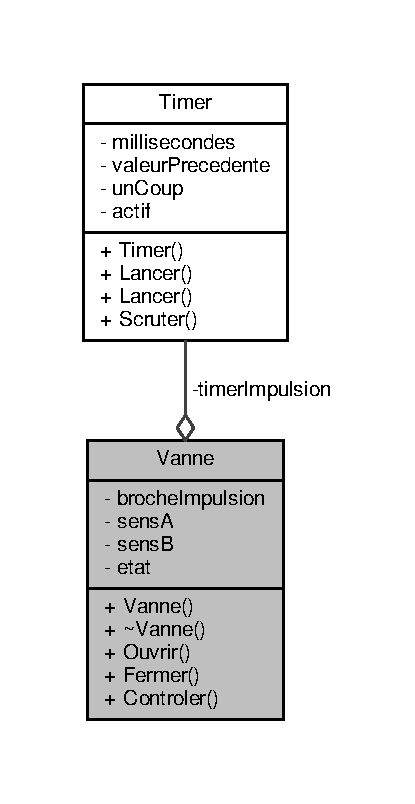
\includegraphics[width=199pt]{class_vanne__coll__graph}
\end{center}
\end{figure}
\subsection*{Types publics}
\begin{DoxyCompactItemize}
\item 
enum \hyperlink{class_vanne_a81379125f1e1526fbb5f07e234736a3f}{E\+T\+A\+T\+\_\+\+V\+A\+N\+NE} \{ \\*
\hyperlink{class_vanne_a81379125f1e1526fbb5f07e234736a3fae109e58f9fd0e71c014508f1d0c0c822}{R\+E\+P\+OS}, 
\hyperlink{class_vanne_a81379125f1e1526fbb5f07e234736a3fa21e006590946195e7563b566ddbb7729}{O\+U\+V\+E\+RT}, 
\hyperlink{class_vanne_a81379125f1e1526fbb5f07e234736a3fa300ae1e445c61cb33a96a6e5724a2390}{F\+E\+R\+M\+ER}, 
\hyperlink{class_vanne_a81379125f1e1526fbb5f07e234736a3fadcc6f97225703ab20b0d0b9bd8a2cc63}{E\+N\+\_\+\+O\+U\+V\+E\+R\+T\+U\+RE}, 
\\*
\hyperlink{class_vanne_a81379125f1e1526fbb5f07e234736a3fa366b255b6287261305630772bf87809f}{E\+N\+\_\+\+F\+E\+R\+M\+E\+T\+U\+RE}, 
\hyperlink{class_vanne_a81379125f1e1526fbb5f07e234736a3fa8e1beadd18316dfa66296a0f5be1bf8f}{E\+N\+\_\+\+A\+T\+T\+E\+N\+T\+E\+\_\+\+O\+U\+V\+E\+R\+T\+U\+RE}, 
\hyperlink{class_vanne_a81379125f1e1526fbb5f07e234736a3fa07fbc78323cdb789ea97d714778e2b19}{E\+N\+\_\+\+A\+T\+T\+E\+N\+T\+E\+\_\+\+F\+E\+R\+M\+E\+T\+U\+RE}
 \}
\end{DoxyCompactItemize}
\subsection*{Fonctions membres publiques}
\begin{DoxyCompactItemize}
\item 
\hyperlink{class_vanne_aa809c804e63bec235b0733091217bdd5}{Vanne} (gpio\+\_\+num\+\_\+t \+\_\+broche\+Impulsion)
\begin{DoxyCompactList}\small\item\em \hyperlink{class_vanne_aa809c804e63bec235b0733091217bdd5}{Vanne\+::\+Vanne}  \+\_\+broche\+Impulsion, c\textquotesingle{}est le numéro de la broche sur laquelle on enverra l\textquotesingle{}impulsion. \end{DoxyCompactList}\item 
virtual \hyperlink{class_vanne_a682923104515512c227d3a91c5f156ed}{$\sim$\+Vanne} ()
\item 
void \hyperlink{class_vanne_abaf4f1253b0fb8016b86280017a5fd53}{Ouvrir} ()
\begin{DoxyCompactList}\small\item\em \hyperlink{class_vanne_abaf4f1253b0fb8016b86280017a5fd53}{Vanne\+::\+Ouvrir}. \end{DoxyCompactList}\item 
void \hyperlink{class_vanne_a009f9021ff1f44fa633eee3e8f42bd9f}{Fermer} ()
\begin{DoxyCompactList}\small\item\em \hyperlink{class_vanne_a009f9021ff1f44fa633eee3e8f42bd9f}{Vanne\+::\+Fermer}. \end{DoxyCompactList}\item 
int \hyperlink{class_vanne_a81820af5e718ed19bb3d7359484c8b88}{Controler} (char commande)
\begin{DoxyCompactList}\small\item\em \hyperlink{class_vanne_a81820af5e718ed19bb3d7359484c8b88}{Vanne\+::\+Controler}. \end{DoxyCompactList}\end{DoxyCompactItemize}
\subsection*{Attributs privés}
\begin{DoxyCompactItemize}
\item 
gpio\+\_\+num\+\_\+t \hyperlink{class_vanne_a972da53e393d5b1911b2c1bff2fc0cc7}{broche\+Impulsion}
\item 
\hyperlink{class_timer}{Timer} \hyperlink{class_vanne_a3cc616e595d81a083fe79dc1a5a74fa2}{timer\+Impulsion}
\item 
const gpio\+\_\+num\+\_\+t \hyperlink{class_vanne_ae5e8b2f4a69751a996ff535ff56c44bf}{sensA}
\item 
const gpio\+\_\+num\+\_\+t \hyperlink{class_vanne_ad50ee3497ec27d35b52b17531f0019b3}{sensB}
\item 
\hyperlink{class_vanne_a81379125f1e1526fbb5f07e234736a3f}{E\+T\+A\+T\+\_\+\+V\+A\+N\+NE} \hyperlink{class_vanne_aeb49318747b8a7cb8eeb3f9b9e6a3c71}{etat}
\end{DoxyCompactItemize}


\subsection{Documentation des énumérations membres}
\index{Vanne@{Vanne}!E\+T\+A\+T\+\_\+\+V\+A\+N\+NE@{E\+T\+A\+T\+\_\+\+V\+A\+N\+NE}}
\index{E\+T\+A\+T\+\_\+\+V\+A\+N\+NE@{E\+T\+A\+T\+\_\+\+V\+A\+N\+NE}!Vanne@{Vanne}}
\subsubsection[{\texorpdfstring{E\+T\+A\+T\+\_\+\+V\+A\+N\+NE}{ETAT_VANNE}}]{\setlength{\rightskip}{0pt plus 5cm}enum {\bf Vanne\+::\+E\+T\+A\+T\+\_\+\+V\+A\+N\+NE}}\hypertarget{class_vanne_a81379125f1e1526fbb5f07e234736a3f}{}\label{class_vanne_a81379125f1e1526fbb5f07e234736a3f}
\begin{Desc}
\item[Valeurs énumérées]\par
\begin{description}
\index{R\+E\+P\+OS@{R\+E\+P\+OS}!Vanne@{Vanne}}\index{Vanne@{Vanne}!R\+E\+P\+OS@{R\+E\+P\+OS}}\item[{\em 
R\+E\+P\+OS\hypertarget{class_vanne_a81379125f1e1526fbb5f07e234736a3fae109e58f9fd0e71c014508f1d0c0c822}{}\label{class_vanne_a81379125f1e1526fbb5f07e234736a3fae109e58f9fd0e71c014508f1d0c0c822}
}]\index{O\+U\+V\+E\+RT@{O\+U\+V\+E\+RT}!Vanne@{Vanne}}\index{Vanne@{Vanne}!O\+U\+V\+E\+RT@{O\+U\+V\+E\+RT}}\item[{\em 
O\+U\+V\+E\+RT\hypertarget{class_vanne_a81379125f1e1526fbb5f07e234736a3fa21e006590946195e7563b566ddbb7729}{}\label{class_vanne_a81379125f1e1526fbb5f07e234736a3fa21e006590946195e7563b566ddbb7729}
}]\index{F\+E\+R\+M\+ER@{F\+E\+R\+M\+ER}!Vanne@{Vanne}}\index{Vanne@{Vanne}!F\+E\+R\+M\+ER@{F\+E\+R\+M\+ER}}\item[{\em 
F\+E\+R\+M\+ER\hypertarget{class_vanne_a81379125f1e1526fbb5f07e234736a3fa300ae1e445c61cb33a96a6e5724a2390}{}\label{class_vanne_a81379125f1e1526fbb5f07e234736a3fa300ae1e445c61cb33a96a6e5724a2390}
}]\index{E\+N\+\_\+\+O\+U\+V\+E\+R\+T\+U\+RE@{E\+N\+\_\+\+O\+U\+V\+E\+R\+T\+U\+RE}!Vanne@{Vanne}}\index{Vanne@{Vanne}!E\+N\+\_\+\+O\+U\+V\+E\+R\+T\+U\+RE@{E\+N\+\_\+\+O\+U\+V\+E\+R\+T\+U\+RE}}\item[{\em 
E\+N\+\_\+\+O\+U\+V\+E\+R\+T\+U\+RE\hypertarget{class_vanne_a81379125f1e1526fbb5f07e234736a3fadcc6f97225703ab20b0d0b9bd8a2cc63}{}\label{class_vanne_a81379125f1e1526fbb5f07e234736a3fadcc6f97225703ab20b0d0b9bd8a2cc63}
}]\index{E\+N\+\_\+\+F\+E\+R\+M\+E\+T\+U\+RE@{E\+N\+\_\+\+F\+E\+R\+M\+E\+T\+U\+RE}!Vanne@{Vanne}}\index{Vanne@{Vanne}!E\+N\+\_\+\+F\+E\+R\+M\+E\+T\+U\+RE@{E\+N\+\_\+\+F\+E\+R\+M\+E\+T\+U\+RE}}\item[{\em 
E\+N\+\_\+\+F\+E\+R\+M\+E\+T\+U\+RE\hypertarget{class_vanne_a81379125f1e1526fbb5f07e234736a3fa366b255b6287261305630772bf87809f}{}\label{class_vanne_a81379125f1e1526fbb5f07e234736a3fa366b255b6287261305630772bf87809f}
}]\index{E\+N\+\_\+\+A\+T\+T\+E\+N\+T\+E\+\_\+\+O\+U\+V\+E\+R\+T\+U\+RE@{E\+N\+\_\+\+A\+T\+T\+E\+N\+T\+E\+\_\+\+O\+U\+V\+E\+R\+T\+U\+RE}!Vanne@{Vanne}}\index{Vanne@{Vanne}!E\+N\+\_\+\+A\+T\+T\+E\+N\+T\+E\+\_\+\+O\+U\+V\+E\+R\+T\+U\+RE@{E\+N\+\_\+\+A\+T\+T\+E\+N\+T\+E\+\_\+\+O\+U\+V\+E\+R\+T\+U\+RE}}\item[{\em 
E\+N\+\_\+\+A\+T\+T\+E\+N\+T\+E\+\_\+\+O\+U\+V\+E\+R\+T\+U\+RE\hypertarget{class_vanne_a81379125f1e1526fbb5f07e234736a3fa8e1beadd18316dfa66296a0f5be1bf8f}{}\label{class_vanne_a81379125f1e1526fbb5f07e234736a3fa8e1beadd18316dfa66296a0f5be1bf8f}
}]\index{E\+N\+\_\+\+A\+T\+T\+E\+N\+T\+E\+\_\+\+F\+E\+R\+M\+E\+T\+U\+RE@{E\+N\+\_\+\+A\+T\+T\+E\+N\+T\+E\+\_\+\+F\+E\+R\+M\+E\+T\+U\+RE}!Vanne@{Vanne}}\index{Vanne@{Vanne}!E\+N\+\_\+\+A\+T\+T\+E\+N\+T\+E\+\_\+\+F\+E\+R\+M\+E\+T\+U\+RE@{E\+N\+\_\+\+A\+T\+T\+E\+N\+T\+E\+\_\+\+F\+E\+R\+M\+E\+T\+U\+RE}}\item[{\em 
E\+N\+\_\+\+A\+T\+T\+E\+N\+T\+E\+\_\+\+F\+E\+R\+M\+E\+T\+U\+RE\hypertarget{class_vanne_a81379125f1e1526fbb5f07e234736a3fa07fbc78323cdb789ea97d714778e2b19}{}\label{class_vanne_a81379125f1e1526fbb5f07e234736a3fa07fbc78323cdb789ea97d714778e2b19}
}]\end{description}
\end{Desc}


\subsection{Documentation des constructeurs et destructeur}
\index{Vanne@{Vanne}!Vanne@{Vanne}}
\index{Vanne@{Vanne}!Vanne@{Vanne}}
\subsubsection[{\texorpdfstring{Vanne(gpio\+\_\+num\+\_\+t \+\_\+broche\+Impulsion)}{Vanne(gpio_num_t _brocheImpulsion)}}]{\setlength{\rightskip}{0pt plus 5cm}Vanne\+::\+Vanne (
\begin{DoxyParamCaption}
\item[{gpio\+\_\+num\+\_\+t}]{\+\_\+broche\+Impulsion}
\end{DoxyParamCaption}
)}\hypertarget{class_vanne_aa809c804e63bec235b0733091217bdd5}{}\label{class_vanne_aa809c804e63bec235b0733091217bdd5}


\hyperlink{class_vanne_aa809c804e63bec235b0733091217bdd5}{Vanne\+::\+Vanne}  \+\_\+broche\+Impulsion, c\textquotesingle{}est le numéro de la broche sur laquelle on enverra l\textquotesingle{}impulsion. 

Constructeur de la classe. \index{Vanne@{Vanne}!````~Vanne@{$\sim$\+Vanne}}
\index{````~Vanne@{$\sim$\+Vanne}!Vanne@{Vanne}}
\subsubsection[{\texorpdfstring{$\sim$\+Vanne()}{~Vanne()}}]{\setlength{\rightskip}{0pt plus 5cm}Vanne\+::$\sim$\+Vanne (
\begin{DoxyParamCaption}
{}
\end{DoxyParamCaption}
)\hspace{0.3cm}{\ttfamily [virtual]}}\hypertarget{class_vanne_a682923104515512c227d3a91c5f156ed}{}\label{class_vanne_a682923104515512c227d3a91c5f156ed}


\subsection{Documentation des fonctions membres}
\index{Vanne@{Vanne}!Controler@{Controler}}
\index{Controler@{Controler}!Vanne@{Vanne}}
\subsubsection[{\texorpdfstring{Controler(char commande)}{Controler(char commande)}}]{\setlength{\rightskip}{0pt plus 5cm}int Vanne\+::\+Controler (
\begin{DoxyParamCaption}
\item[{char}]{commande}
\end{DoxyParamCaption}
)}\hypertarget{class_vanne_a81820af5e718ed19bb3d7359484c8b88}{}\label{class_vanne_a81820af5e718ed19bb3d7359484c8b88}


\hyperlink{class_vanne_a81820af5e718ed19bb3d7359484c8b88}{Vanne\+::\+Controler}. 


\begin{DoxyParams}{Paramètres}
{\em char} & commande\\
\hline
\end{DoxyParams}
On va regarder l\textquotesingle{}état de la vanne et effectuer une action en fonction de son état. \index{Vanne@{Vanne}!Fermer@{Fermer}}
\index{Fermer@{Fermer}!Vanne@{Vanne}}
\subsubsection[{\texorpdfstring{Fermer()}{Fermer()}}]{\setlength{\rightskip}{0pt plus 5cm}void Vanne\+::\+Fermer (
\begin{DoxyParamCaption}
{}
\end{DoxyParamCaption}
)}\hypertarget{class_vanne_a009f9021ff1f44fa633eee3e8f42bd9f}{}\label{class_vanne_a009f9021ff1f44fa633eee3e8f42bd9f}


\hyperlink{class_vanne_a009f9021ff1f44fa633eee3e8f42bd9f}{Vanne\+::\+Fermer}. 

Si il n\textquotesingle{}y a pas de mutex alors on configure les broches en fermeture et on lance le Timer\+Impulsion pendant 250ms

Sinon, on attend la fermeture \index{Vanne@{Vanne}!Ouvrir@{Ouvrir}}
\index{Ouvrir@{Ouvrir}!Vanne@{Vanne}}
\subsubsection[{\texorpdfstring{Ouvrir()}{Ouvrir()}}]{\setlength{\rightskip}{0pt plus 5cm}void Vanne\+::\+Ouvrir (
\begin{DoxyParamCaption}
{}
\end{DoxyParamCaption}
)}\hypertarget{class_vanne_abaf4f1253b0fb8016b86280017a5fd53}{}\label{class_vanne_abaf4f1253b0fb8016b86280017a5fd53}


\hyperlink{class_vanne_abaf4f1253b0fb8016b86280017a5fd53}{Vanne\+::\+Ouvrir}. 

Si il n\textquotesingle{}y a pas de mutex alors on configure les broches en ouverture et on lance le Timer\+Impulsion pendant 250ms

Sinon, on attend l\textquotesingle{}ouverture 

\subsection{Documentation des données membres}
\index{Vanne@{Vanne}!broche\+Impulsion@{broche\+Impulsion}}
\index{broche\+Impulsion@{broche\+Impulsion}!Vanne@{Vanne}}
\subsubsection[{\texorpdfstring{broche\+Impulsion}{brocheImpulsion}}]{\setlength{\rightskip}{0pt plus 5cm}gpio\+\_\+num\+\_\+t Vanne\+::broche\+Impulsion\hspace{0.3cm}{\ttfamily [private]}}\hypertarget{class_vanne_a972da53e393d5b1911b2c1bff2fc0cc7}{}\label{class_vanne_a972da53e393d5b1911b2c1bff2fc0cc7}
\index{Vanne@{Vanne}!etat@{etat}}
\index{etat@{etat}!Vanne@{Vanne}}
\subsubsection[{\texorpdfstring{etat}{etat}}]{\setlength{\rightskip}{0pt plus 5cm}{\bf E\+T\+A\+T\+\_\+\+V\+A\+N\+NE} Vanne\+::etat\hspace{0.3cm}{\ttfamily [private]}}\hypertarget{class_vanne_aeb49318747b8a7cb8eeb3f9b9e6a3c71}{}\label{class_vanne_aeb49318747b8a7cb8eeb3f9b9e6a3c71}
\index{Vanne@{Vanne}!sensA@{sensA}}
\index{sensA@{sensA}!Vanne@{Vanne}}
\subsubsection[{\texorpdfstring{sensA}{sensA}}]{\setlength{\rightskip}{0pt plus 5cm}const gpio\+\_\+num\+\_\+t Vanne\+::sensA\hspace{0.3cm}{\ttfamily [private]}}\hypertarget{class_vanne_ae5e8b2f4a69751a996ff535ff56c44bf}{}\label{class_vanne_ae5e8b2f4a69751a996ff535ff56c44bf}
\index{Vanne@{Vanne}!sensB@{sensB}}
\index{sensB@{sensB}!Vanne@{Vanne}}
\subsubsection[{\texorpdfstring{sensB}{sensB}}]{\setlength{\rightskip}{0pt plus 5cm}const gpio\+\_\+num\+\_\+t Vanne\+::sensB\hspace{0.3cm}{\ttfamily [private]}}\hypertarget{class_vanne_ad50ee3497ec27d35b52b17531f0019b3}{}\label{class_vanne_ad50ee3497ec27d35b52b17531f0019b3}
\index{Vanne@{Vanne}!timer\+Impulsion@{timer\+Impulsion}}
\index{timer\+Impulsion@{timer\+Impulsion}!Vanne@{Vanne}}
\subsubsection[{\texorpdfstring{timer\+Impulsion}{timerImpulsion}}]{\setlength{\rightskip}{0pt plus 5cm}{\bf Timer} Vanne\+::timer\+Impulsion\hspace{0.3cm}{\ttfamily [private]}}\hypertarget{class_vanne_a3cc616e595d81a083fe79dc1a5a74fa2}{}\label{class_vanne_a3cc616e595d81a083fe79dc1a5a74fa2}


La documentation de cette classe a été générée à partir des fichiers suivants \+:\begin{DoxyCompactItemize}
\item 
\hyperlink{vanne_8h}{vanne.\+h}\item 
\hyperlink{vanne_8cpp}{vanne.\+cpp}\end{DoxyCompactItemize}

\hypertarget{class_zone}{}\section{Référence de la classe Zone}
\label{class_zone}\index{Zone@{Zone}}


{\ttfamily \#include $<$zone.\+h$>$}



Graphe de collaboration de Zone\+:\nopagebreak
\begin{figure}[H]
\begin{center}
\leavevmode
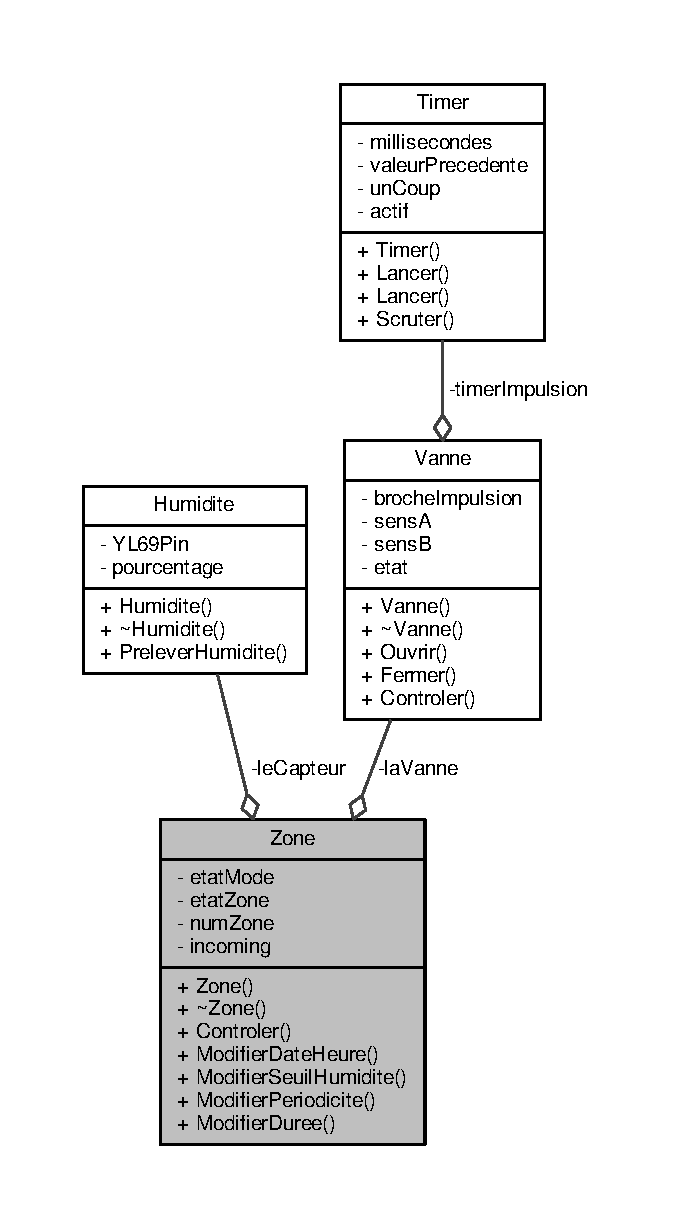
\includegraphics[height=550pt]{class_zone__coll__graph}
\end{center}
\end{figure}
\subsection*{Types publics}
\begin{DoxyCompactItemize}
\item 
enum \hyperlink{class_zone_a07d053965fa6722cfc3f80d225677497}{M\+O\+D\+E\+\_\+\+Z\+O\+NE} \{ \hyperlink{class_zone_a07d053965fa6722cfc3f80d225677497a3c754e4a55948ba52fb8329c2874e54d}{M\+O\+D\+E\+\_\+\+M\+A\+N\+U\+EL}, 
\hyperlink{class_zone_a07d053965fa6722cfc3f80d225677497a95a13ba1fd5830ac255f4cc762e0261a}{M\+O\+D\+E\+\_\+\+P\+R\+O\+G\+R\+A\+M\+ME}, 
\hyperlink{class_zone_a07d053965fa6722cfc3f80d225677497a337c2f25b250da75f6590ba4735a19df}{M\+O\+D\+E\+\_\+\+A\+U\+T\+O\+M\+A\+T\+I\+Q\+UE}
 \}
\item 
enum \hyperlink{class_zone_afed66edb8ab1446dcab5186028648880}{E\+T\+A\+T\+\_\+\+Z\+O\+NE} \{ \hyperlink{class_zone_afed66edb8ab1446dcab5186028648880ab0e5fa888d8db41efd00d61e527e80d3}{A\+T\+T\+E\+N\+TE}, 
\hyperlink{class_zone_afed66edb8ab1446dcab5186028648880ac2006f5be5833d01d79c46e0878e581d}{O\+U\+V\+E\+R\+T\+U\+RE}, 
\hyperlink{class_zone_afed66edb8ab1446dcab5186028648880ac566eede85c70a9ecd7555dfe1df9871}{F\+E\+R\+M\+E\+T\+U\+RE}
 \}
\end{DoxyCompactItemize}
\subsection*{Fonctions membres publiques}
\begin{DoxyCompactItemize}
\item 
\hyperlink{class_zone_ae3e1df767b1138077d5a0c4b60b6be10}{Zone} (int nb\+Zone, gpio\+\_\+num\+\_\+t \+\_\+commande\+Vanne, gpio\+\_\+num\+\_\+t \+\_\+broche\+Humidite)
\begin{DoxyCompactList}\small\item\em \hyperlink{class_zone_ae3e1df767b1138077d5a0c4b60b6be10}{Zone\+::\+Zone}. \end{DoxyCompactList}\item 
\hyperlink{class_zone_a562607cb5c4120a9316c5e967a5c610b}{$\sim$\+Zone} ()
\begin{DoxyCompactList}\small\item\em \hyperlink{class_zone_a562607cb5c4120a9316c5e967a5c610b}{Zone\+::$\sim$\+Zone}. \end{DoxyCompactList}\item 
int \hyperlink{class_zone_a27c5d83a0f4a2c965cbf0b8ae5c5bd9e}{Controler} (String \+\_\+parametre)
\begin{DoxyCompactList}\small\item\em \hyperlink{class_zone_a27c5d83a0f4a2c965cbf0b8ae5c5bd9e}{Zone\+::\+Controler}. \end{DoxyCompactList}\item 
int \hyperlink{class_zone_aeb1ceb3e614cbfcd53e9565f6afefb59}{Modifier\+Date\+Heure} ()
\item 
int \hyperlink{class_zone_a1f6fc952bc1ceb3acda81669ce875c04}{Modifier\+Seuil\+Humidite} ()
\item 
int \hyperlink{class_zone_ade9182f137c6db1c7c29a7b367991c3d}{Modifier\+Periodicite} ()
\item 
int \hyperlink{class_zone_a4390b52a1631ec05bc3a796db50bc5dd}{Modifier\+Duree} ()
\end{DoxyCompactItemize}
\subsection*{Attributs privés}
\begin{DoxyCompactItemize}
\item 
\hyperlink{class_zone_a07d053965fa6722cfc3f80d225677497}{M\+O\+D\+E\+\_\+\+Z\+O\+NE} \hyperlink{class_zone_aa5e3a0305eda31639e37736109b7c957}{etat\+Mode}
\item 
\hyperlink{class_zone_afed66edb8ab1446dcab5186028648880}{E\+T\+A\+T\+\_\+\+Z\+O\+NE} \hyperlink{class_zone_a6130d56057619acb91ecce2a465b3b20}{etat\+Zone}
\item 
int \hyperlink{class_zone_a0efa38f2d12ae4d9ffcbffdee9b4f438}{num\+Zone}
\item 
String \hyperlink{class_zone_ac4e36c704602ec1d06d90a1f2c62b8be}{incoming}
\item 
\hyperlink{class_vanne}{Vanne} \hyperlink{class_zone_a375ebd280cc5bd60ba3e76a36224bc44}{la\+Vanne}
\item 
\hyperlink{class_humidite}{Humidite} \hyperlink{class_zone_a1f070429b7b55eb43aed46664f64f469}{le\+Capteur}
\end{DoxyCompactItemize}


\subsection{Documentation des énumérations membres}
\index{Zone@{Zone}!E\+T\+A\+T\+\_\+\+Z\+O\+NE@{E\+T\+A\+T\+\_\+\+Z\+O\+NE}}
\index{E\+T\+A\+T\+\_\+\+Z\+O\+NE@{E\+T\+A\+T\+\_\+\+Z\+O\+NE}!Zone@{Zone}}
\subsubsection[{\texorpdfstring{E\+T\+A\+T\+\_\+\+Z\+O\+NE}{ETAT_ZONE}}]{\setlength{\rightskip}{0pt plus 5cm}enum {\bf Zone\+::\+E\+T\+A\+T\+\_\+\+Z\+O\+NE}}\hypertarget{class_zone_afed66edb8ab1446dcab5186028648880}{}\label{class_zone_afed66edb8ab1446dcab5186028648880}
\begin{Desc}
\item[Valeurs énumérées]\par
\begin{description}
\index{A\+T\+T\+E\+N\+TE@{A\+T\+T\+E\+N\+TE}!Zone@{Zone}}\index{Zone@{Zone}!A\+T\+T\+E\+N\+TE@{A\+T\+T\+E\+N\+TE}}\item[{\em 
A\+T\+T\+E\+N\+TE\hypertarget{class_zone_afed66edb8ab1446dcab5186028648880ab0e5fa888d8db41efd00d61e527e80d3}{}\label{class_zone_afed66edb8ab1446dcab5186028648880ab0e5fa888d8db41efd00d61e527e80d3}
}]\index{O\+U\+V\+E\+R\+T\+U\+RE@{O\+U\+V\+E\+R\+T\+U\+RE}!Zone@{Zone}}\index{Zone@{Zone}!O\+U\+V\+E\+R\+T\+U\+RE@{O\+U\+V\+E\+R\+T\+U\+RE}}\item[{\em 
O\+U\+V\+E\+R\+T\+U\+RE\hypertarget{class_zone_afed66edb8ab1446dcab5186028648880ac2006f5be5833d01d79c46e0878e581d}{}\label{class_zone_afed66edb8ab1446dcab5186028648880ac2006f5be5833d01d79c46e0878e581d}
}]\index{F\+E\+R\+M\+E\+T\+U\+RE@{F\+E\+R\+M\+E\+T\+U\+RE}!Zone@{Zone}}\index{Zone@{Zone}!F\+E\+R\+M\+E\+T\+U\+RE@{F\+E\+R\+M\+E\+T\+U\+RE}}\item[{\em 
F\+E\+R\+M\+E\+T\+U\+RE\hypertarget{class_zone_afed66edb8ab1446dcab5186028648880ac566eede85c70a9ecd7555dfe1df9871}{}\label{class_zone_afed66edb8ab1446dcab5186028648880ac566eede85c70a9ecd7555dfe1df9871}
}]\end{description}
\end{Desc}
\index{Zone@{Zone}!M\+O\+D\+E\+\_\+\+Z\+O\+NE@{M\+O\+D\+E\+\_\+\+Z\+O\+NE}}
\index{M\+O\+D\+E\+\_\+\+Z\+O\+NE@{M\+O\+D\+E\+\_\+\+Z\+O\+NE}!Zone@{Zone}}
\subsubsection[{\texorpdfstring{M\+O\+D\+E\+\_\+\+Z\+O\+NE}{MODE_ZONE}}]{\setlength{\rightskip}{0pt plus 5cm}enum {\bf Zone\+::\+M\+O\+D\+E\+\_\+\+Z\+O\+NE}}\hypertarget{class_zone_a07d053965fa6722cfc3f80d225677497}{}\label{class_zone_a07d053965fa6722cfc3f80d225677497}
\begin{Desc}
\item[Valeurs énumérées]\par
\begin{description}
\index{M\+O\+D\+E\+\_\+\+M\+A\+N\+U\+EL@{M\+O\+D\+E\+\_\+\+M\+A\+N\+U\+EL}!Zone@{Zone}}\index{Zone@{Zone}!M\+O\+D\+E\+\_\+\+M\+A\+N\+U\+EL@{M\+O\+D\+E\+\_\+\+M\+A\+N\+U\+EL}}\item[{\em 
M\+O\+D\+E\+\_\+\+M\+A\+N\+U\+EL\hypertarget{class_zone_a07d053965fa6722cfc3f80d225677497a3c754e4a55948ba52fb8329c2874e54d}{}\label{class_zone_a07d053965fa6722cfc3f80d225677497a3c754e4a55948ba52fb8329c2874e54d}
}]\index{M\+O\+D\+E\+\_\+\+P\+R\+O\+G\+R\+A\+M\+ME@{M\+O\+D\+E\+\_\+\+P\+R\+O\+G\+R\+A\+M\+ME}!Zone@{Zone}}\index{Zone@{Zone}!M\+O\+D\+E\+\_\+\+P\+R\+O\+G\+R\+A\+M\+ME@{M\+O\+D\+E\+\_\+\+P\+R\+O\+G\+R\+A\+M\+ME}}\item[{\em 
M\+O\+D\+E\+\_\+\+P\+R\+O\+G\+R\+A\+M\+ME\hypertarget{class_zone_a07d053965fa6722cfc3f80d225677497a95a13ba1fd5830ac255f4cc762e0261a}{}\label{class_zone_a07d053965fa6722cfc3f80d225677497a95a13ba1fd5830ac255f4cc762e0261a}
}]\index{M\+O\+D\+E\+\_\+\+A\+U\+T\+O\+M\+A\+T\+I\+Q\+UE@{M\+O\+D\+E\+\_\+\+A\+U\+T\+O\+M\+A\+T\+I\+Q\+UE}!Zone@{Zone}}\index{Zone@{Zone}!M\+O\+D\+E\+\_\+\+A\+U\+T\+O\+M\+A\+T\+I\+Q\+UE@{M\+O\+D\+E\+\_\+\+A\+U\+T\+O\+M\+A\+T\+I\+Q\+UE}}\item[{\em 
M\+O\+D\+E\+\_\+\+A\+U\+T\+O\+M\+A\+T\+I\+Q\+UE\hypertarget{class_zone_a07d053965fa6722cfc3f80d225677497a337c2f25b250da75f6590ba4735a19df}{}\label{class_zone_a07d053965fa6722cfc3f80d225677497a337c2f25b250da75f6590ba4735a19df}
}]\end{description}
\end{Desc}


\subsection{Documentation des constructeurs et destructeur}
\index{Zone@{Zone}!Zone@{Zone}}
\index{Zone@{Zone}!Zone@{Zone}}
\subsubsection[{\texorpdfstring{Zone(int nb\+Zone, gpio\+\_\+num\+\_\+t \+\_\+commande\+Vanne, gpio\+\_\+num\+\_\+t \+\_\+broche\+Humidite)}{Zone(int nbZone, gpio_num_t _commandeVanne, gpio_num_t _brocheHumidite)}}]{\setlength{\rightskip}{0pt plus 5cm}Zone\+::\+Zone (
\begin{DoxyParamCaption}
\item[{int}]{nb\+Zone, }
\item[{gpio\+\_\+num\+\_\+t}]{\+\_\+commande\+Vanne, }
\item[{gpio\+\_\+num\+\_\+t}]{\+\_\+broche\+Humidite}
\end{DoxyParamCaption}
)}\hypertarget{class_zone_ae3e1df767b1138077d5a0c4b60b6be10}{}\label{class_zone_ae3e1df767b1138077d5a0c4b60b6be10}


\hyperlink{class_zone_ae3e1df767b1138077d5a0c4b60b6be10}{Zone\+::\+Zone}. 


\begin{DoxyParams}{Paramètres}
{\em int} & nb\+Zone permet de connaitre le nom de la zone \\
\hline
{\em gpio\+\_\+num\+\_\+t} & \+\_\+commande\+Vanne c\textquotesingle{}est la broche de la vanne à gérer \\
\hline
{\em gpio\+\_\+num\+\_\+t} & \+\_\+broche\+Humidite, c\textquotesingle{}est la broche du capteur d\textquotesingle{}humidité\\
\hline
\end{DoxyParams}
Constructeur de la classe. \index{Zone@{Zone}!````~Zone@{$\sim$\+Zone}}
\index{````~Zone@{$\sim$\+Zone}!Zone@{Zone}}
\subsubsection[{\texorpdfstring{$\sim$\+Zone()}{~Zone()}}]{\setlength{\rightskip}{0pt plus 5cm}Zone\+::$\sim$\+Zone (
\begin{DoxyParamCaption}
{}
\end{DoxyParamCaption}
)}\hypertarget{class_zone_a562607cb5c4120a9316c5e967a5c610b}{}\label{class_zone_a562607cb5c4120a9316c5e967a5c610b}


\hyperlink{class_zone_a562607cb5c4120a9316c5e967a5c610b}{Zone\+::$\sim$\+Zone}. 

Déstructeur de la classe. 

\subsection{Documentation des fonctions membres}
\index{Zone@{Zone}!Controler@{Controler}}
\index{Controler@{Controler}!Zone@{Zone}}
\subsubsection[{\texorpdfstring{Controler(\+String \+\_\+parametre)}{Controler(String _parametre)}}]{\setlength{\rightskip}{0pt plus 5cm}int Zone\+::\+Controler (
\begin{DoxyParamCaption}
\item[{String}]{\+\_\+parametre}
\end{DoxyParamCaption}
)}\hypertarget{class_zone_a27c5d83a0f4a2c965cbf0b8ae5c5bd9e}{}\label{class_zone_a27c5d83a0f4a2c965cbf0b8ae5c5bd9e}


\hyperlink{class_zone_a27c5d83a0f4a2c965cbf0b8ae5c5bd9e}{Zone\+::\+Controler}. 


\begin{DoxyParams}{Paramètres}
{\em string} & \+\_\+parametre, c\textquotesingle{}est la chaine que renvoie l\textquotesingle{}application lorsqu\textquotesingle{}une action est effectuée\\
\hline
\end{DoxyParams}
Si la chaine de caractère reçue commence par un m, alors on passe en mode manuel et l\textquotesingle{}ouverture ou la fermeture dependera du caractère suivant.

Si elle commence par un p on passe en mode programmé et si elle commence par un a alors on passe en mode auto. \index{Zone@{Zone}!Modifier\+Date\+Heure@{Modifier\+Date\+Heure}}
\index{Modifier\+Date\+Heure@{Modifier\+Date\+Heure}!Zone@{Zone}}
\subsubsection[{\texorpdfstring{Modifier\+Date\+Heure()}{ModifierDateHeure()}}]{\setlength{\rightskip}{0pt plus 5cm}int Zone\+::\+Modifier\+Date\+Heure (
\begin{DoxyParamCaption}
{}
\end{DoxyParamCaption}
)}\hypertarget{class_zone_aeb1ceb3e614cbfcd53e9565f6afefb59}{}\label{class_zone_aeb1ceb3e614cbfcd53e9565f6afefb59}
\index{Zone@{Zone}!Modifier\+Duree@{Modifier\+Duree}}
\index{Modifier\+Duree@{Modifier\+Duree}!Zone@{Zone}}
\subsubsection[{\texorpdfstring{Modifier\+Duree()}{ModifierDuree()}}]{\setlength{\rightskip}{0pt plus 5cm}int Zone\+::\+Modifier\+Duree (
\begin{DoxyParamCaption}
{}
\end{DoxyParamCaption}
)}\hypertarget{class_zone_a4390b52a1631ec05bc3a796db50bc5dd}{}\label{class_zone_a4390b52a1631ec05bc3a796db50bc5dd}
\index{Zone@{Zone}!Modifier\+Periodicite@{Modifier\+Periodicite}}
\index{Modifier\+Periodicite@{Modifier\+Periodicite}!Zone@{Zone}}
\subsubsection[{\texorpdfstring{Modifier\+Periodicite()}{ModifierPeriodicite()}}]{\setlength{\rightskip}{0pt plus 5cm}int Zone\+::\+Modifier\+Periodicite (
\begin{DoxyParamCaption}
{}
\end{DoxyParamCaption}
)}\hypertarget{class_zone_ade9182f137c6db1c7c29a7b367991c3d}{}\label{class_zone_ade9182f137c6db1c7c29a7b367991c3d}
\index{Zone@{Zone}!Modifier\+Seuil\+Humidite@{Modifier\+Seuil\+Humidite}}
\index{Modifier\+Seuil\+Humidite@{Modifier\+Seuil\+Humidite}!Zone@{Zone}}
\subsubsection[{\texorpdfstring{Modifier\+Seuil\+Humidite()}{ModifierSeuilHumidite()}}]{\setlength{\rightskip}{0pt plus 5cm}int Zone\+::\+Modifier\+Seuil\+Humidite (
\begin{DoxyParamCaption}
{}
\end{DoxyParamCaption}
)}\hypertarget{class_zone_a1f6fc952bc1ceb3acda81669ce875c04}{}\label{class_zone_a1f6fc952bc1ceb3acda81669ce875c04}


\subsection{Documentation des données membres}
\index{Zone@{Zone}!etat\+Mode@{etat\+Mode}}
\index{etat\+Mode@{etat\+Mode}!Zone@{Zone}}
\subsubsection[{\texorpdfstring{etat\+Mode}{etatMode}}]{\setlength{\rightskip}{0pt plus 5cm}{\bf M\+O\+D\+E\+\_\+\+Z\+O\+NE} Zone\+::etat\+Mode\hspace{0.3cm}{\ttfamily [private]}}\hypertarget{class_zone_aa5e3a0305eda31639e37736109b7c957}{}\label{class_zone_aa5e3a0305eda31639e37736109b7c957}
\index{Zone@{Zone}!etat\+Zone@{etat\+Zone}}
\index{etat\+Zone@{etat\+Zone}!Zone@{Zone}}
\subsubsection[{\texorpdfstring{etat\+Zone}{etatZone}}]{\setlength{\rightskip}{0pt plus 5cm}{\bf E\+T\+A\+T\+\_\+\+Z\+O\+NE} Zone\+::etat\+Zone\hspace{0.3cm}{\ttfamily [private]}}\hypertarget{class_zone_a6130d56057619acb91ecce2a465b3b20}{}\label{class_zone_a6130d56057619acb91ecce2a465b3b20}
\index{Zone@{Zone}!incoming@{incoming}}
\index{incoming@{incoming}!Zone@{Zone}}
\subsubsection[{\texorpdfstring{incoming}{incoming}}]{\setlength{\rightskip}{0pt plus 5cm}String Zone\+::incoming\hspace{0.3cm}{\ttfamily [private]}}\hypertarget{class_zone_ac4e36c704602ec1d06d90a1f2c62b8be}{}\label{class_zone_ac4e36c704602ec1d06d90a1f2c62b8be}
\index{Zone@{Zone}!la\+Vanne@{la\+Vanne}}
\index{la\+Vanne@{la\+Vanne}!Zone@{Zone}}
\subsubsection[{\texorpdfstring{la\+Vanne}{laVanne}}]{\setlength{\rightskip}{0pt plus 5cm}{\bf Vanne} Zone\+::la\+Vanne\hspace{0.3cm}{\ttfamily [private]}}\hypertarget{class_zone_a375ebd280cc5bd60ba3e76a36224bc44}{}\label{class_zone_a375ebd280cc5bd60ba3e76a36224bc44}
\index{Zone@{Zone}!le\+Capteur@{le\+Capteur}}
\index{le\+Capteur@{le\+Capteur}!Zone@{Zone}}
\subsubsection[{\texorpdfstring{le\+Capteur}{leCapteur}}]{\setlength{\rightskip}{0pt plus 5cm}{\bf Humidite} Zone\+::le\+Capteur\hspace{0.3cm}{\ttfamily [private]}}\hypertarget{class_zone_a1f070429b7b55eb43aed46664f64f469}{}\label{class_zone_a1f070429b7b55eb43aed46664f64f469}
\index{Zone@{Zone}!num\+Zone@{num\+Zone}}
\index{num\+Zone@{num\+Zone}!Zone@{Zone}}
\subsubsection[{\texorpdfstring{num\+Zone}{numZone}}]{\setlength{\rightskip}{0pt plus 5cm}int Zone\+::num\+Zone\hspace{0.3cm}{\ttfamily [private]}}\hypertarget{class_zone_a0efa38f2d12ae4d9ffcbffdee9b4f438}{}\label{class_zone_a0efa38f2d12ae4d9ffcbffdee9b4f438}


La documentation de cette classe a été générée à partir des fichiers suivants \+:\begin{DoxyCompactItemize}
\item 
\hyperlink{zone_8h}{zone.\+h}\item 
\hyperlink{zone_8cpp}{zone.\+cpp}\end{DoxyCompactItemize}

\chapter{Documentation des fichiers}
\hypertarget{controleur_de_serre_8cpp}{}\section{Référence du fichier controleur\+De\+Serre.\+cpp}
\label{controleur_de_serre_8cpp}\index{controleur\+De\+Serre.\+cpp@{controleur\+De\+Serre.\+cpp}}
{\ttfamily \#include \char`\"{}controleur\+De\+Serre.\+h\char`\"{}}\\*
Graphe des dépendances par inclusion de controleur\+De\+Serre.\+cpp\+:\nopagebreak
\begin{figure}[H]
\begin{center}
\leavevmode
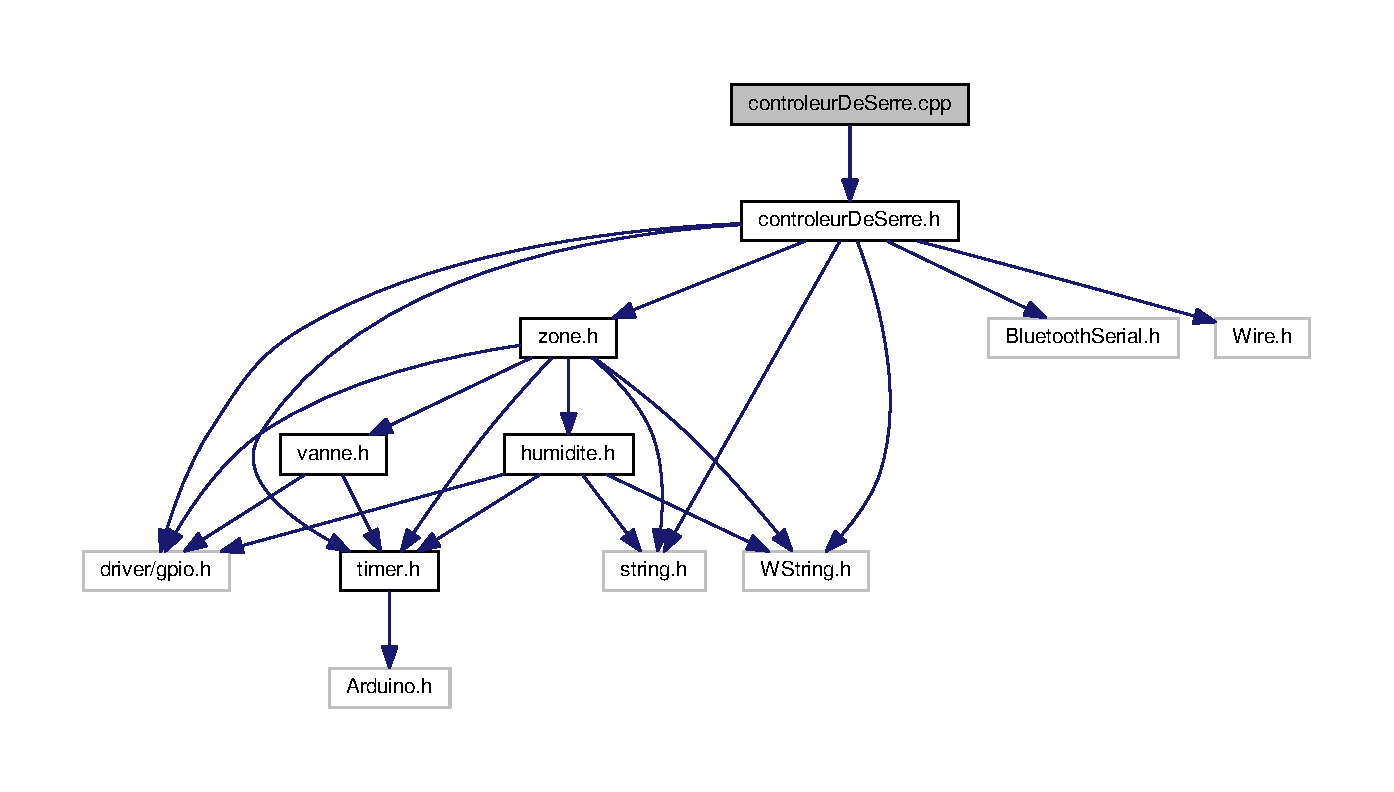
\includegraphics[width=350pt]{controleur_de_serre_8cpp__incl}
\end{center}
\end{figure}


\subsection{Description détaillée}
\begin{DoxyAuthor}{Auteur}
Michaud théo 
\end{DoxyAuthor}
\begin{DoxyDate}{Date}
Vendredi 15 avril 2019 
\end{DoxyDate}

\hypertarget{controleur_de_serre_8h}{}\section{Référence du fichier controleur\+De\+Serre.\+h}
\label{controleur_de_serre_8h}\index{controleur\+De\+Serre.\+h@{controleur\+De\+Serre.\+h}}
{\ttfamily \#include $<$driver/gpio.\+h$>$}\\*
{\ttfamily \#include $<$string.\+h$>$}\\*
{\ttfamily \#include \char`\"{}timer.\+h\char`\"{}}\\*
{\ttfamily \#include $<$W\+String.\+h$>$}\\*
{\ttfamily \#include \char`\"{}Bluetooth\+Serial.\+h\char`\"{}}\\*
{\ttfamily \#include $<$Wire.\+h$>$}\\*
{\ttfamily \#include \char`\"{}zone.\+h\char`\"{}}\\*
Graphe des dépendances par inclusion de controleur\+De\+Serre.\+h\+:\nopagebreak
\begin{figure}[H]
\begin{center}
\leavevmode
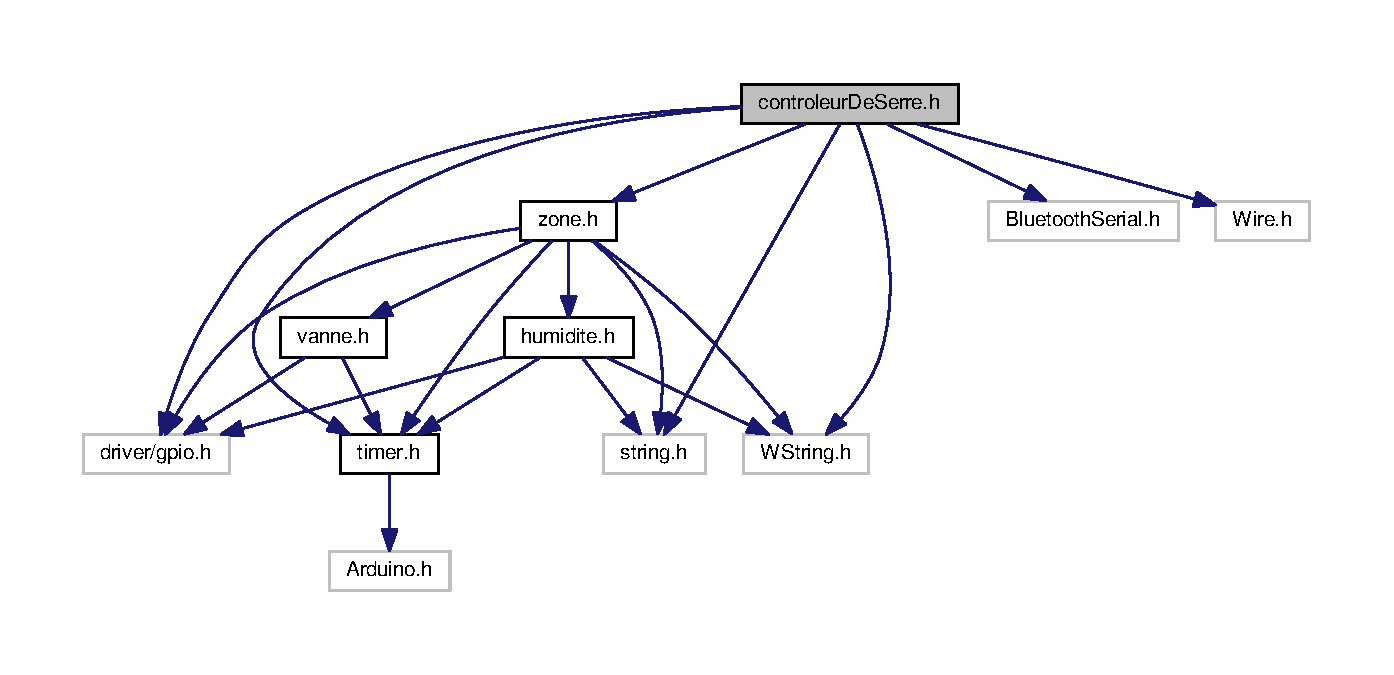
\includegraphics[width=350pt]{controleur_de_serre_8h__incl}
\end{center}
\end{figure}
Ce graphe montre quels fichiers incluent directement ou indirectement ce fichier \+:\nopagebreak
\begin{figure}[H]
\begin{center}
\leavevmode
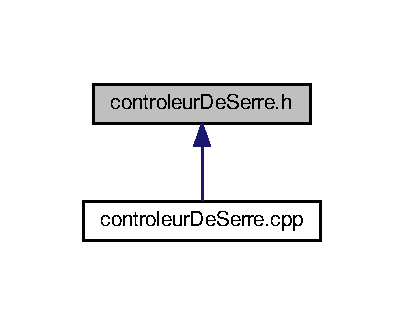
\includegraphics[width=194pt]{controleur_de_serre_8h__dep__incl}
\end{center}
\end{figure}
\subsection*{Classes}
\begin{DoxyCompactItemize}
\item 
class \hyperlink{class_controleur_de_serre}{Controleur\+De\+Serre}
\end{DoxyCompactItemize}


\subsection{Description détaillée}
\begin{DoxyAuthor}{Auteur}
Michaud théo 
\end{DoxyAuthor}
\begin{DoxyDate}{Date}
Vendredi 15 avril 2019 
\end{DoxyDate}

\hypertarget{humidite_8cpp}{}\section{Référence du fichier humidite.\+cpp}
\label{humidite_8cpp}\index{humidite.\+cpp@{humidite.\+cpp}}
{\ttfamily \#include \char`\"{}humidite.\+h\char`\"{}}\\*
{\ttfamily \#include \char`\"{}timer.\+h\char`\"{}}\\*
Graphe des dépendances par inclusion de humidite.\+cpp\+:\nopagebreak
\begin{figure}[H]
\begin{center}
\leavevmode
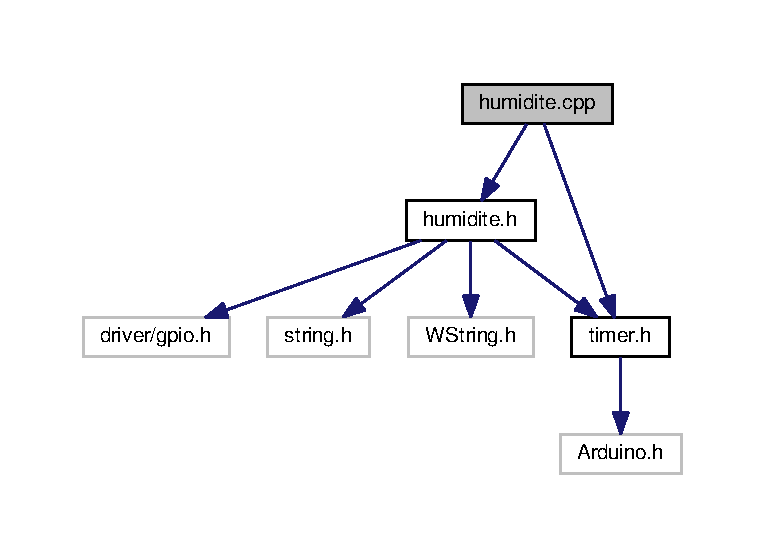
\includegraphics[width=350pt]{humidite_8cpp__incl}
\end{center}
\end{figure}
\subsection*{Variables}
\begin{DoxyCompactItemize}
\item 
\hyperlink{class_timer}{Timer} \hyperlink{humidite_8cpp_a3a0ecca60fe446194daf5a3cf2addeb6}{timer\+Attentes}
\end{DoxyCompactItemize}


\subsection{Description détaillée}
\begin{DoxyAuthor}{Auteur}
Michaud théo 
\end{DoxyAuthor}
\begin{DoxyDate}{Date}
Vendredi 15 avril 2019 
\end{DoxyDate}


\subsection{Documentation des variables}
\index{humidite.\+cpp@{humidite.\+cpp}!timer\+Attentes@{timer\+Attentes}}
\index{timer\+Attentes@{timer\+Attentes}!humidite.\+cpp@{humidite.\+cpp}}
\subsubsection[{\texorpdfstring{timer\+Attentes}{timerAttentes}}]{\setlength{\rightskip}{0pt plus 5cm}{\bf Timer} timer\+Attentes}\hypertarget{humidite_8cpp_a3a0ecca60fe446194daf5a3cf2addeb6}{}\label{humidite_8cpp_a3a0ecca60fe446194daf5a3cf2addeb6}

\hypertarget{humidite_8h}{}\section{Référence du fichier humidite.\+h}
\label{humidite_8h}\index{humidite.\+h@{humidite.\+h}}
{\ttfamily \#include $<$driver/gpio.\+h$>$}\\*
{\ttfamily \#include $<$string.\+h$>$}\\*
{\ttfamily \#include \char`\"{}timer.\+h\char`\"{}}\\*
{\ttfamily \#include $<$W\+String.\+h$>$}\\*
Graphe des dépendances par inclusion de humidite.\+h\+:\nopagebreak
\begin{figure}[H]
\begin{center}
\leavevmode
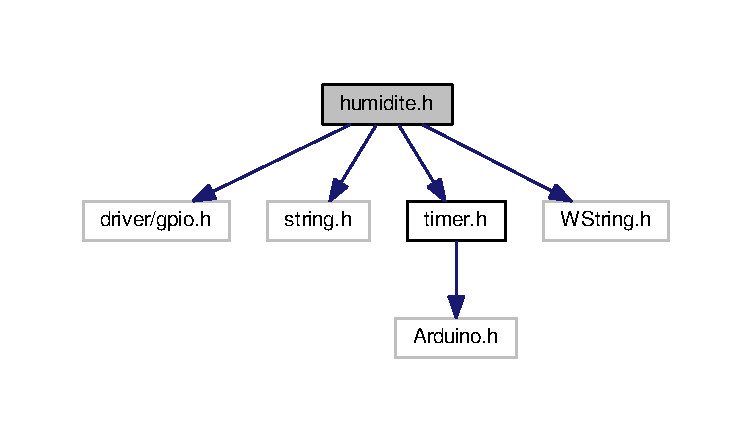
\includegraphics[width=350pt]{humidite_8h__incl}
\end{center}
\end{figure}
Ce graphe montre quels fichiers incluent directement ou indirectement ce fichier \+:\nopagebreak
\begin{figure}[H]
\begin{center}
\leavevmode
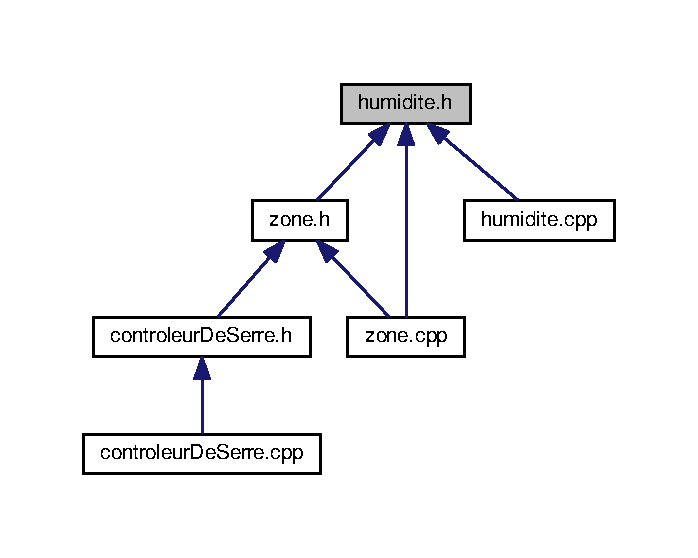
\includegraphics[width=335pt]{humidite_8h__dep__incl}
\end{center}
\end{figure}
\subsection*{Classes}
\begin{DoxyCompactItemize}
\item 
class \hyperlink{class_humidite}{Humidite}
\end{DoxyCompactItemize}


\subsection{Description détaillée}
\begin{DoxyAuthor}{Auteur}
Michaud théo 
\end{DoxyAuthor}
\begin{DoxyDate}{Date}
Vendredi 15 avril 2019 
\end{DoxyDate}

\hypertarget{timer_8cpp}{}\section{Référence du fichier timer.\+cpp}
\label{timer_8cpp}\index{timer.\+cpp@{timer.\+cpp}}
{\ttfamily \#include \char`\"{}timer.\+h\char`\"{}}\\*
Graphe des dépendances par inclusion de timer.\+cpp\+:\nopagebreak
\begin{figure}[H]
\begin{center}
\leavevmode
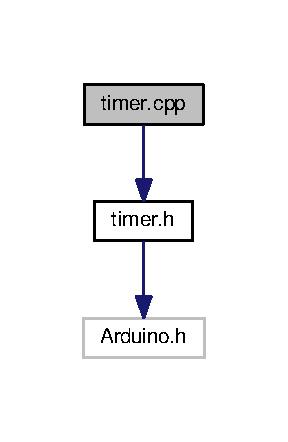
\includegraphics[width=138pt]{timer_8cpp__incl}
\end{center}
\end{figure}


\subsection{Description détaillée}
\begin{DoxyAuthor}{Auteur}
Michaud théo 
\end{DoxyAuthor}
\begin{DoxyDate}{Date}
Vendredi 29 mars 2019 
\end{DoxyDate}

\hypertarget{timer_8h}{}\section{Référence du fichier timer.\+h}
\label{timer_8h}\index{timer.\+h@{timer.\+h}}
{\ttfamily \#include $<$Arduino.\+h$>$}\\*
Graphe des dépendances par inclusion de timer.\+h\+:\nopagebreak
\begin{figure}[H]
\begin{center}
\leavevmode
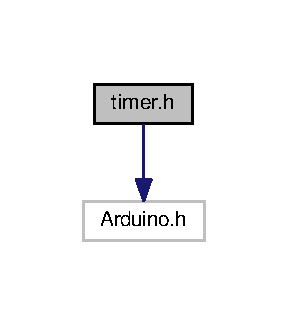
\includegraphics[width=138pt]{timer_8h__incl}
\end{center}
\end{figure}
Ce graphe montre quels fichiers incluent directement ou indirectement ce fichier \+:\nopagebreak
\begin{figure}[H]
\begin{center}
\leavevmode
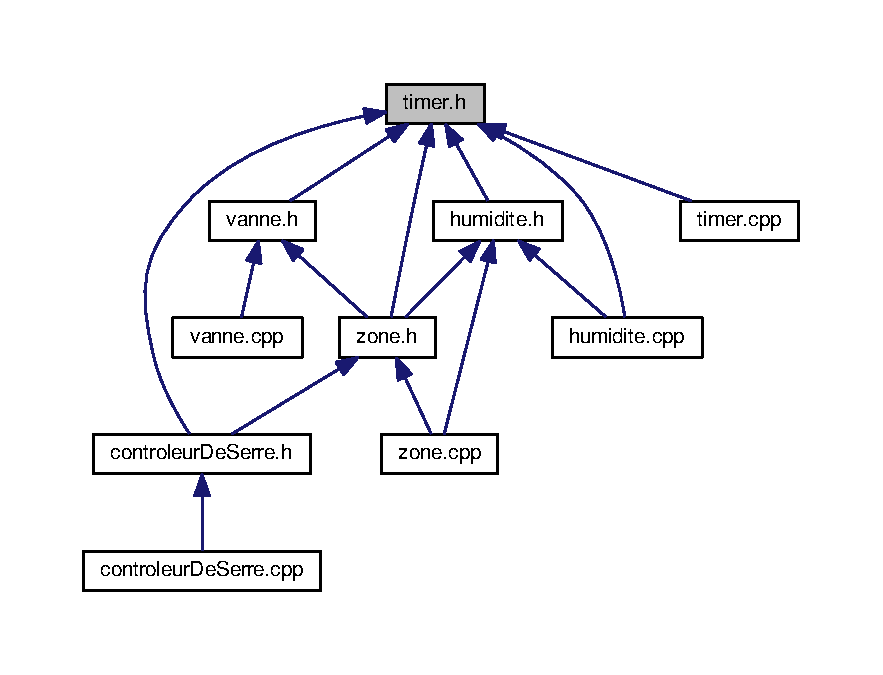
\includegraphics[width=350pt]{timer_8h__dep__incl}
\end{center}
\end{figure}
\subsection*{Classes}
\begin{DoxyCompactItemize}
\item 
class \hyperlink{class_timer}{Timer}
\end{DoxyCompactItemize}


\subsection{Description détaillée}
\begin{DoxyAuthor}{Auteur}
Michaud Théo 
\end{DoxyAuthor}
\begin{DoxyDate}{Date}
Vendredi 29 mars 2019 
\end{DoxyDate}

\hypertarget{vanne_8cpp}{}\section{Référence du fichier vanne.\+cpp}
\label{vanne_8cpp}\index{vanne.\+cpp@{vanne.\+cpp}}
{\ttfamily \#include \char`\"{}vanne.\+h\char`\"{}}\\*
Graphe des dépendances par inclusion de vanne.\+cpp\+:\nopagebreak
\begin{figure}[H]
\begin{center}
\leavevmode
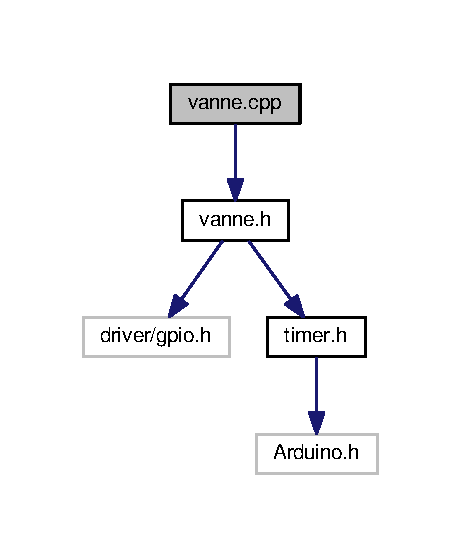
\includegraphics[width=221pt]{vanne_8cpp__incl}
\end{center}
\end{figure}
\subsection*{Variables}
\begin{DoxyCompactItemize}
\item 
bool \hyperlink{vanne_8cpp_afe182008b150b20d224c757ba2d86094}{mutex} = false
\end{DoxyCompactItemize}


\subsection{Description détaillée}
\begin{DoxyAuthor}{Auteur}
Michaud théo 
\end{DoxyAuthor}
\begin{DoxyDate}{Date}
Vendredi 15 mars 2019 
\end{DoxyDate}


\subsection{Documentation des variables}
\index{vanne.\+cpp@{vanne.\+cpp}!mutex@{mutex}}
\index{mutex@{mutex}!vanne.\+cpp@{vanne.\+cpp}}
\subsubsection[{\texorpdfstring{mutex}{mutex}}]{\setlength{\rightskip}{0pt plus 5cm}bool mutex = false}\hypertarget{vanne_8cpp_afe182008b150b20d224c757ba2d86094}{}\label{vanne_8cpp_afe182008b150b20d224c757ba2d86094}

\hypertarget{vanne_8h}{}\section{Référence du fichier vanne.\+h}
\label{vanne_8h}\index{vanne.\+h@{vanne.\+h}}
{\ttfamily \#include $<$driver/gpio.\+h$>$}\\*
{\ttfamily \#include \char`\"{}timer.\+h\char`\"{}}\\*
Graphe des dépendances par inclusion de vanne.\+h\+:\nopagebreak
\begin{figure}[H]
\begin{center}
\leavevmode
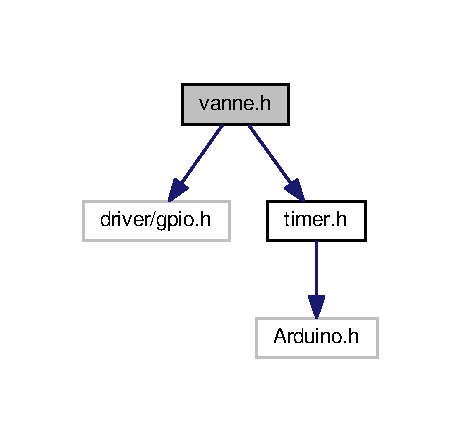
\includegraphics[width=221pt]{vanne_8h__incl}
\end{center}
\end{figure}
Ce graphe montre quels fichiers incluent directement ou indirectement ce fichier \+:\nopagebreak
\begin{figure}[H]
\begin{center}
\leavevmode
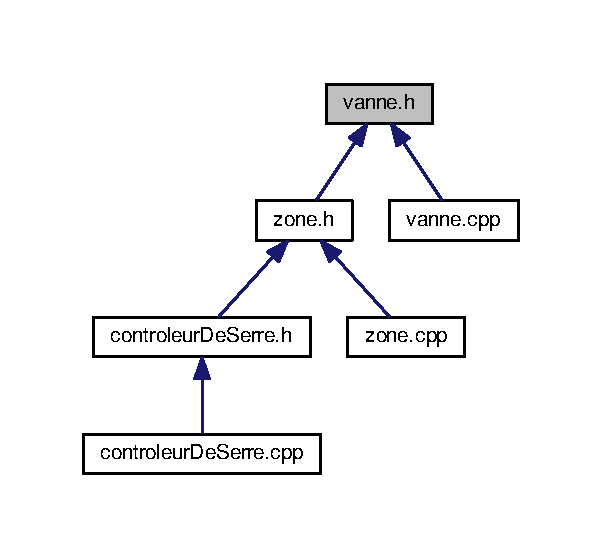
\includegraphics[width=289pt]{vanne_8h__dep__incl}
\end{center}
\end{figure}
\subsection*{Classes}
\begin{DoxyCompactItemize}
\item 
class \hyperlink{class_vanne}{Vanne}
\end{DoxyCompactItemize}
\subsection*{Macros}
\begin{DoxyCompactItemize}
\item 
\#define \hyperlink{vanne_8h_a72cd57a20f51fc921c1f4d3c3303e426}{S\+E\+N\+S\+\_\+A}~G\+P\+I\+O\+\_\+\+N\+U\+M\+\_\+16
\item 
\#define \hyperlink{vanne_8h_ab395814c8c7799f4f4ed3192a7af0284}{S\+E\+N\+S\+\_\+B}~G\+P\+I\+O\+\_\+\+N\+U\+M\+\_\+17
\end{DoxyCompactItemize}


\subsection{Description détaillée}
\begin{DoxyAuthor}{Auteur}
Michaud théo 
\end{DoxyAuthor}
\begin{DoxyDate}{Date}
Vendredi 15 mars 2019 
\end{DoxyDate}


\subsection{Documentation des macros}
\index{vanne.\+h@{vanne.\+h}!S\+E\+N\+S\+\_\+A@{S\+E\+N\+S\+\_\+A}}
\index{S\+E\+N\+S\+\_\+A@{S\+E\+N\+S\+\_\+A}!vanne.\+h@{vanne.\+h}}
\subsubsection[{\texorpdfstring{S\+E\+N\+S\+\_\+A}{SENS_A}}]{\setlength{\rightskip}{0pt plus 5cm}\#define S\+E\+N\+S\+\_\+A~G\+P\+I\+O\+\_\+\+N\+U\+M\+\_\+16}\hypertarget{vanne_8h_a72cd57a20f51fc921c1f4d3c3303e426}{}\label{vanne_8h_a72cd57a20f51fc921c1f4d3c3303e426}
\index{vanne.\+h@{vanne.\+h}!S\+E\+N\+S\+\_\+B@{S\+E\+N\+S\+\_\+B}}
\index{S\+E\+N\+S\+\_\+B@{S\+E\+N\+S\+\_\+B}!vanne.\+h@{vanne.\+h}}
\subsubsection[{\texorpdfstring{S\+E\+N\+S\+\_\+B}{SENS_B}}]{\setlength{\rightskip}{0pt plus 5cm}\#define S\+E\+N\+S\+\_\+B~G\+P\+I\+O\+\_\+\+N\+U\+M\+\_\+17}\hypertarget{vanne_8h_ab395814c8c7799f4f4ed3192a7af0284}{}\label{vanne_8h_ab395814c8c7799f4f4ed3192a7af0284}

\hypertarget{zone_8cpp}{}\section{Référence du fichier zone.\+cpp}
\label{zone_8cpp}\index{zone.\+cpp@{zone.\+cpp}}
{\ttfamily \#include \char`\"{}zone.\+h\char`\"{}}\\*
{\ttfamily \#include $<$Arduino.\+h$>$}\\*
{\ttfamily \#include \char`\"{}humidite.\+h\char`\"{}}\\*
Graphe des dépendances par inclusion de zone.\+cpp\+:\nopagebreak
\begin{figure}[H]
\begin{center}
\leavevmode
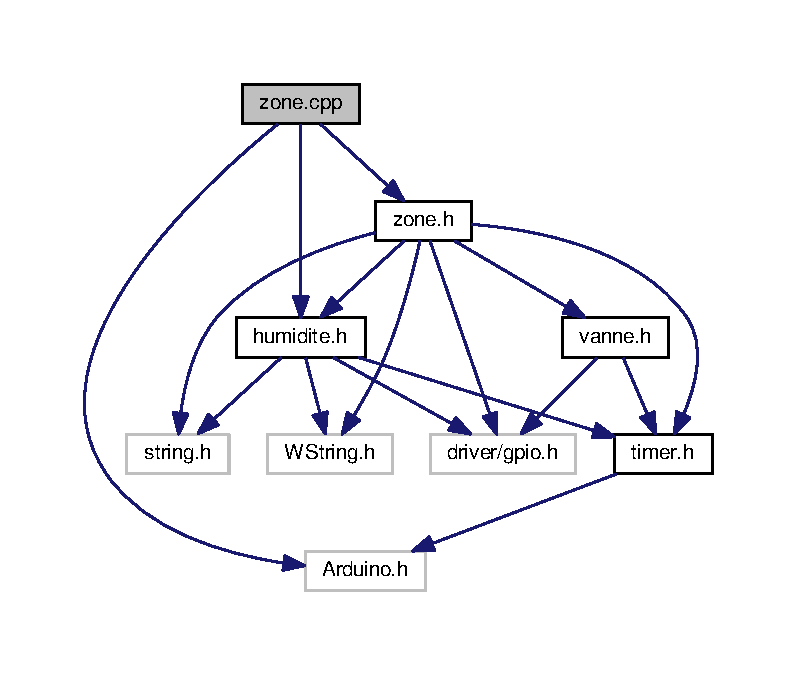
\includegraphics[width=350pt]{zone_8cpp__incl}
\end{center}
\end{figure}


\subsection{Description détaillée}
\begin{DoxyAuthor}{Auteur}
Michaud théo 
\end{DoxyAuthor}
\begin{DoxyDate}{Date}
Vendredi 10 avril 2019 
\end{DoxyDate}

\hypertarget{zone_8h}{}\section{Référence du fichier zone.\+h}
\label{zone_8h}\index{zone.\+h@{zone.\+h}}
{\ttfamily \#include $<$driver/gpio.\+h$>$}\\*
{\ttfamily \#include $<$string.\+h$>$}\\*
{\ttfamily \#include \char`\"{}timer.\+h\char`\"{}}\\*
{\ttfamily \#include $<$W\+String.\+h$>$}\\*
{\ttfamily \#include \char`\"{}vanne.\+h\char`\"{}}\\*
{\ttfamily \#include \char`\"{}humidite.\+h\char`\"{}}\\*
Graphe des dépendances par inclusion de zone.\+h\+:\nopagebreak
\begin{figure}[H]
\begin{center}
\leavevmode
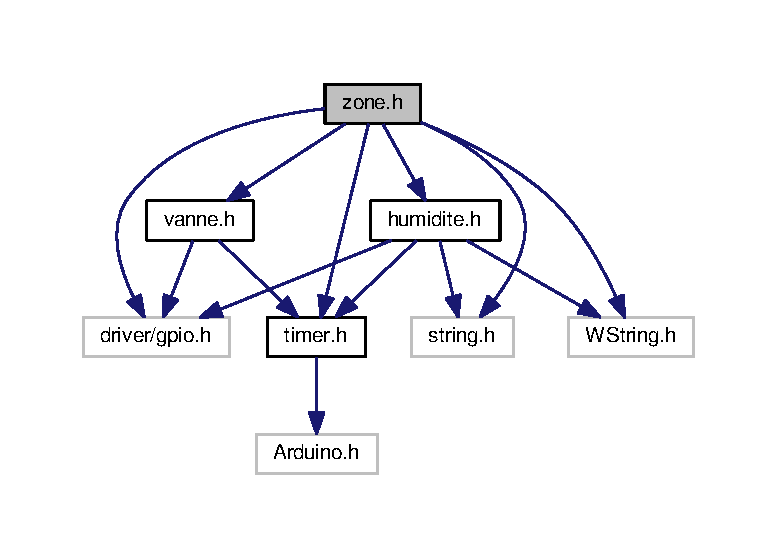
\includegraphics[width=350pt]{zone_8h__incl}
\end{center}
\end{figure}
Ce graphe montre quels fichiers incluent directement ou indirectement ce fichier \+:\nopagebreak
\begin{figure}[H]
\begin{center}
\leavevmode
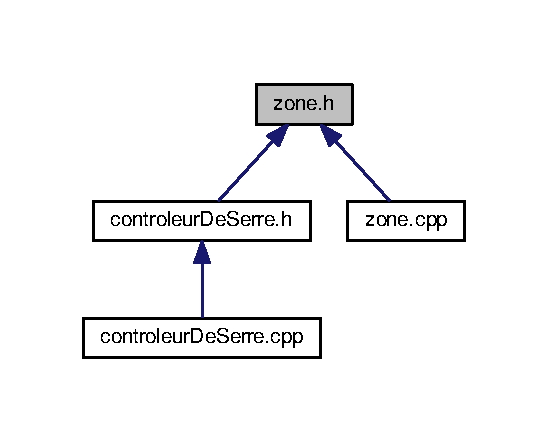
\includegraphics[width=263pt]{zone_8h__dep__incl}
\end{center}
\end{figure}
\subsection*{Classes}
\begin{DoxyCompactItemize}
\item 
class \hyperlink{class_zone}{Zone}
\end{DoxyCompactItemize}


\subsection{Description détaillée}
\begin{DoxyAuthor}{Auteur}
Michaud théo 
\end{DoxyAuthor}
\begin{DoxyDate}{Date}
Vendredi 10 avril 2019 
\end{DoxyDate}

%--- End generated contents ---

% Index
\backmatter
\newpage
\phantomsection
\clearemptydoublepage
\addcontentsline{toc}{chapter}{Index}
\printindex

\end{document}
